\documentclass[conference,10pt,letterpaper]{IEEEtran}

\newif\ifShowLog
\ShowLogfalse

\usepackage[utf8]{inputenc}

% IEEE recommended packages
\usepackage{amsmath}
\interdisplaylinepenalty=2500
\usepackage{algorithmic}
\ifCLASSOPTIONcompsoc
\usepackage[caption=false,font=normalsize,labelfont=sf,textfont=sf]{subfig}
\else
\usepackage[caption=false,font=footnotesize]{subfig}
\fi
\usepackage{dblfloatfix}
\usepackage{url}

% custom packages
\usepackage{amssymb}
\usepackage{verbatim}
\usepackage{soul}
\usepackage{paralist}

\usepackage[usenames,dvipsnames]{xcolor}
\usepackage{colortbl}
\definecolor{TableRowGray}{gray}{0.93}

\usepackage{tikz}
\usetikzlibrary{shadows}
\usepackage{pgfplots}
\pgfplotsset{compat=1.10}

\definecolor{blueLine}{RGB}{57,106,177}
\definecolor{blueFill}{RGB}{114,147,203}
\definecolor{redLine}{RGB}{204,37,41}
\definecolor{greenline}{RGB}{0,250,0}
\definecolor{blackLine}{RGB}{0,0,0}
\definecolor{goldLine}{RGB}{160,82,45}


\usepackage{listings}%

\usepackage[textsize=tiny, textwidth=1.5cm,disable]{todonotes}
%\usepackage{marginnote} 
%\let\marginpar\marginnote

\newcommand{\Abhishek}[1]{\todo[color=yellow!50, linecolor=black!50,inline]{\textbf{Abhishek}: #1}}
\newcommand{\AbhishekC}[1]{\todo[color=yellow!50, linecolor=black!50]{\textbf{Abhishek}: #1}}

\newcommand{\Karla}[1]{\todo[color=green!30, linecolor=black!50,inline]{\textbf{Karla}: #1}}
\newcommand{\KarlaC}[1]{\todo[color=green!30, linecolor=black!50]{\textbf{Karla}: #1}}

\newcommand{\Aron}[1]{\todo[color=blue!10, linecolor=black!50,inline]{\textbf{Aron}: #1}}
\newcommand{\AronC}[1]{\todo[color=blue!10, linecolor=black!50]{\textbf{Aron}: #1}}

\newcommand{\Mike}[1]{\todo[color=orange!30, linecolor=black!50,inline]{\textbf{Mike}: #1}}
\newcommand{\MikeC}[1]{\todo[color=orange!30, linecolor=black!50]{\textbf{Mike}: #1}}

\newcommand{\scott}[1]{\todo[color=purple!30, linecolor=black!50,inline]{\textbf{Scott}: #1}}
\newcommand{\scottC}[1]{\todo[color=purple!30, linecolor=black!50]{\textbf{Scott}: #1}}

\begin{document}
\setlength{\marginparwidth}{1.5cm} % THIS IS REQUIRED FOR THE CORRECT PLACEMENT OF TODONOTES MARGIN NOTES

\title{Design and Implementation of Safe and Private Forward-Trading Platform for\\ IoT-Based Transactive Microgrids}

\author{\IEEEauthorblockN{Aron Laszka}
\IEEEauthorblockA{University of Houston}\\
%\IEEEauthorblockN{Monika Sturm}
%\IEEEauthorblockA{Siemens Corporate Technology}
\and
\IEEEauthorblockN{Abhishek Dubey}
\IEEEauthorblockA{Vanderbilt University}
\and
\IEEEauthorblockN{Scott Eisele}
\IEEEauthorblockA{Vanderbilt University}
\and
\IEEEauthorblockN{Michael Walker}
\IEEEauthorblockA{Vanderbilt University}
\and
\IEEEauthorblockN{Karla Kvaternik}
\IEEEauthorblockA{Siemens Corporate Technology}\\
%\IEEEauthorblockN{Martin Lehofer}
%\IEEEauthorblockA{Siemens Corporate Technology}
}
\renewcommand{\lstlistingname}{log}



\maketitle

% REMOVE BEFORE SUBMISSION!
\thispagestyle{plain}
\pagestyle{plain}

\begin{abstract}
Power grids are undergoing major changes due to rapid growth in renewable energy and improvements in battery technology. Prompted by the increasing complexity of power systems, decentralized IoT solutions are emerging, which arrange local communities into transactive microgrids.
We address the problem of implementing transactive energy mechanisms in a distributed setting, providing both privacy and safety.  Specifically, we design and implement an automated auction and matching system that ensures safety (i.e. satisfaction of line capacity constraints), preserves privacy, and promotes local trade and market efficiency for IoT-based transactive energy systems. This design problem is challenging because safety, market efficiency, and privacy are competing objectives.
We implement our solution as a decentralized IoT-based trading platform, which is built on blockchain technology and smart contracts.
To demonstrate the feasibility of our platform, we perform experiments with dozens of embedded devices and energy production and consumption profiles from a real dataset.
\end{abstract}

\begin{IEEEkeywords}Transactive energy platform, Internet of Things, blockchain, privacy, security, safety, smart contract.\end{IEEEkeywords}

%!TEX root = paper.tex
\section{Introduction}

% What are transactive energy systems
% What is the key challenge : decentralized information architecture
% What is the related research
% What are the contributions of this paper
% What is the outline of this paper

Power grids are undergoing major changes due to rapid
acceleration in renewable energy resources, such as wind and solar power \cite{5430489}. % \cite{EIA2014}
For example, 
$4,\!143$ megawatts of solar panels were installed in the third quarter of 2016 \cite{seia}. This capacity is estimated to grow from 4\% in 2015 to 29\% in 2040 \cite{Randal}. At the same time, battery technology costs per kWh have been dropping significantly \cite{stock2015powerful}, reaching grid parity. % \cite{bronski2015economics}
This massive integration of renewable energy requires detailed information and visibility into all aspects of the network, making it difficult to manage, especially in the presence of variable distributed energy resources \cite{7452738}. Therefore, a different vision for the future of power-grid operations is emerging: a decentralized system in which local communities are arranged in microgrids \cite{rahimi2012transactive}. In this vision, energy generation, transmission, distribution and even storage (e.g., electric vehicles in a community) can be strategically used to balance load and demand spikes. 


Furthering the concept of microgrids, transactive energy models have been proposed to support the next distribution system evolution \cite{kok2016society,cox2013structured,melton2013gridwise}. Transactive energy is a set of market based constructs for dynamically balancing the demand and supply across the electrical infrastructure \cite{melton2013gridwise}. In this approach, customers on the same feeder (i.e. sharing a power line link) can operate in an open market, trading and exchanging generated energy locally. Distribution System Operators (DSO) can be the custodian of this market, while still meeting the net demand \cite{7462854}. For example, the Brooklyn Microgrid, which was developed by LO3 Energy as a pilot project, is a peer-to-peer market for locally generated renewable energy.\footnote{\url{http://brooklynmicrogrid.com/}}

On one hand, transactive energy is a decentralized power system controls problem \cite{7452738}, requiring strategic microgrid control to maintain the stability of the community and the utility. On the other hand, it is a distributed market problem where erroneous as well as malicious transactions can create a gap between demand and supply, eventually destabilizing the system. However, in both cases, this system requires a distributed  infrastructure comprising of smart meters, feeders, smart inverters, utility substations, the utility central offices, and the transmission system operator, which has to provide the necessary computation fabric to support the interplay between the energy control and the fiscal market challenges. 
Recently, demand-response systems have been enabled as applications of IoT in smart grid~\cite{Haider2016166}. Transactive energy systems are the next step for smart grid.
% With the advent of IoT-based solutions in smart-grid  dynamic demand response systems, which are a precursor to transactive sytems have been made possible. 

In general, the focus is now on creating a distributed IoT infrastructure%  comprising of smart meters, feeders, smart inverters, utility substations, the utility central offices, and the transmission system operator
, which provides the necessary computation fabric to support the interplay between energy control and fiscal market challenges, as shown by Volttron \cite{katipamula2016volttron},  OpenFMB \cite{gunthersmart}, and the Resilient Information Architecture Platform for Smart Grid (RIAPS) \cite{eisele2017riaps,Scott2017ICCPS}. For instance, the latter is a distributed IoT  ``operating system'' that provides the foundations for all algorithms, isolates the hardware details from the algorithms, and provides essential mechanisms for resource management, fault tolerance, and security. However, most of these efforts are focusing on the computation and distribution of information and, and they do not provide the key support required to handle the privacy challenges that arise from the required information exchange in this decentralized transactive system. 


In this paper, we assume the existence of the IoT infrastructure and specifically focus on the following privacy challenges.
%
%
% This is where the RIAPS and computing services discussion will be included. However, it does not solve the following challenges, which is the focus of this paper.
%
%\Abhishek{Can we merge this with last paragraph? It seems repetitive.}
%\Aron{I'll probably just remove this.}
%Specifically, 
%in order to take advantage of local energy production and storage capabilities, 
%in order to take advantage of these capabilities, 
%electric grids need to become more decentralized.
%However, a decentralized transactive energy system may pose a much greater threat to prosumers' privacy than existing smart metering systems.
%\Abhishek{We can introduce these bullets by stating that the privacy challenges specifically are (the privacy challenges were mentioned at the end of the paragraph above.)}
\begin{itemize}[itemsep=0.25\parskip,topsep=-0.5\parskip]
\item Firstly, since prosumers\footnote{We refer to customers as \emph{prosumers} to emphasize that they can not only consume energy, but may also produce it.}  may purchase energy from each other in a transactive microgrid, transactions may inadvertently reveal the prosumers' detailed energy usage patterns to other prosumers within the microgrid.
Addressing this issue in a decentralized trading system is quite challenging as it requires hiding the identities of trade partners from each other.
In comparison, secure smart metering reveals the prosumers' energy usage patterns \Abhishek{Earlier we mentioned the challenge of privacy with respect to system operator in the abstract. I think the system operator and provider are the same.  My question and comment were included in the abstract about this.} only to the provider. 
\item Secondly, \Abhishek{Is this not related to the first point? Perhaps the first point can be just about identity and second point can be specifically about consumption patterns.}\Aron{The first point is about to whom information might be leaked, and the second point is about the type of information. I'll make this more clear.} transactions may reveal the future energy usage of a prosumer, which could be used to infer private information.
For example, a smart home may know that its inhabitants will go out in the evening (e.g., by looking at their calendar), and it may trade energy futures accordingly in the morning.
Without adequate privacy measures, these trades may reveal to other prosumers in the microgrid that the inhabitants will not be at home later.
Note that energy futures, whose delivery may happen several hours after when the transaction is made, can play a very important role in predicting and controlling microgrid load.
In comparison, smart metering reveals only current (or past) usage.
\item Thirdly, transactions and energy usage data in a transactive microgrid are much richer sources of information than the simple energy usage data collected by smart meters.
More specifically, the information available in a transactive microgrid is a superset of what is available from smart metering, and it may be used to infer personal information, such as risk propensity and financial standing.
\end{itemize}
\vspace{0.5\parskip}

Before transactive energy system can be deployed in practice, we must address these privacy issues.
However, this is a challenging task, as the system also has to satisfy security and safety requirements, which often conflict with privacy goals.
For example, to prevent a prosumer from destabilizing the grid through careless of malicious energy trading, the system must check all of the prosumer's transactions.
In a decentralized system, this requires disseminating information, which could be used to infer the prosumer's future energy consumption.

\Abhishek{Can we cite an example of such a service?}
\Aron{I am not sure what you mean by ``such a service.''}
\Abhishek{We should connect the paper and our work back to IoT in this paragraph.}
In this paper, we propose a system that enables trading energy futures in a secure and verifiable manner, preserves the prosumers' privacy, and enables the DSO to regulate the trading platform and enforce certain safety rules.
\Aron{Since SIGCHI does not have section numbers, this paragraph, which describes the organization of the paper, is not very clear.}
First, we describe the basic components of a transactive microgrid, and we formulate security, safety, and privacy requirements. 
Then, we introduce a decentralized system for transactive microgrids based on distributed ledgers, and describe in detail the transactions and services that are used to implement this system.
Next, we discuss how the system satisfies the security, safety, and privacy requirements.
Finally, we give a brief overview of related work and offer concluding remarks.



% !TeX root = ICCPS18.tex

%\vspace{-0.2in}
\section{System Model}
\label{sec:system}
We consider a microgrid with a set of feeders arranged in a radial topology.\footnote{The methods developed in this paper are extensible to more general tree topologies involving branching. We work with a radial topology to simplify our notation.} 
A feeder has a fixed set of nodes, each representing a residential load or a combination of load and distributed energy resources (DERs) such as rooftop solar and batteries, as shown in Figure~\ref{fig:microgrid}.
Each node is associated with a participant in the local peer-to-peer energy trading market. There is a distribution system operator (DSO) that also participates in the market, and may thus use the market to incentivize timed energy production within the microgrid to aid in grid stabilization and promotion of related ancillary services \cite{7462854}. In addition, the DSO supplies residual demand not met through the local market.
%Figure \ref{fig:commonsequence} describes a typical trading scenario. 
The participants settle trades in advance, which allows them to schedule their transfer of power into the local distribution system. Alternatively, a mechanism can be responsible for matching the producers and consumers. There are typically three phases in these operations: discovery of compatible offers, matching of buying offers to selling offers (it can be made either by each prosumer individually or by an automated matching mechanism). Once the matching is done, the energy transaction and the financial transaction are then handled at a later time. 

% We assume that Distribution System Operators (DSOs) can act as custodians of this market, while still meeting the net demand in the microgrid \cite{7462854}.



% \begin{figure}[ht]
% \centering
% 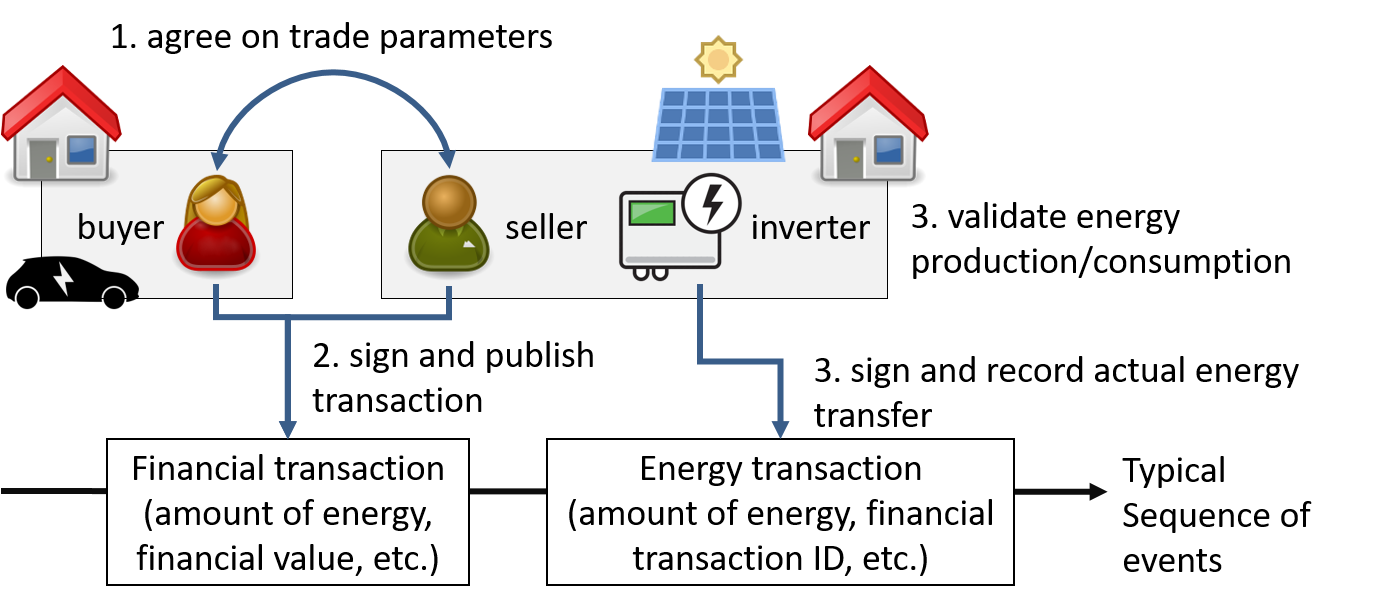
\includegraphics[width=0.5\textwidth]{diagrams/TE.png}
% \caption{A conceptual sequence of activities in a transactive energy system.  %The buyer and seller agree on the trading terms. Then, they do the actual energy transaction.
% %which must be validated.
% %Thereafter, the financial assets are transferred.
% %The red arrows show off-block chain communication and blue arrows show transactions on block-chain. Producers and consumers request the DSO to allocate the energy production and consumption assets to blockchain. The consumers receive asynchronous notification about offers from producers. Thereafter, they can finalize transaction. The energy transfer happens at a later time and is also recorded in the chain. Financial transactions are also done on the blockchain. These financial transactions are later tallied with the energy transactions.\Abhishek{Aron Lets recaption the figure
% }\label{fig:commonsequence}
% \end{figure}


%\AronC{In the problem formulation, we use ``participants'' to refer to all market participants, including the DSO.}. In this formulation, we ignore reactive power.





% \subsection{Transactive Energy Workflow}


% \label{sec:petra}
% %\textcolor{red}{There will be a figure here.}

% \Abhishek{This section should describe a typical transactive energy workflow}
% \AronC{In that case, we could keep Fig.~\ref{fig:petrasequence} and present it as an illustration of a typical workflow.}







%The key aspect of this pattern is the tight integration of distributed  messaging patterns between actors and the blockchain-based communication network used for transferring transactional information. For example, in the transactive energy domain,  
%\Karla{Unfinished sentence}

% In  \cite{Laszka17}, we introduced the key concept of privacy-preserving energy transactions where a consumer selects the producers to trade with. In this basic sequence, the smart contract is  responsible for keeping track of the energy and financial assets enabling producers to post trade offers and exchange assets when a consumer decides to accept. PETra uses quantized energy asset tokens
% %\footnote{There are two kinds of energy tokens: Energy Production Asset and Energy Consumption Asset. Token attributes include power and time interval for which the token is valid.} 
% that can represent the non-negative amount of power to be produced or consumed (for example, measured in watts),  the time interval in which energy is to be produced (or consumed), and the  last time interval in which energy is to be produced (or consumed) (Figure \ref{fig:petrasequence} describes the full sequence of activity)\AronC{Figure \ref{fig:petrasequence} is not an accurate representation of PETra or the Middleware'17 sequence!}.\AbhishekC{Aron please remove this figure and update the sequence} These assets are withdrawn and submitted to anonymized accounts on behalf of prosumers by the DSO, who is also responsible for validating that the specific prosumer has the  energy capacity for feasible trades given the assets. Once the DSO posts the assets into the blockchain, prosumers can trade between themselves using these quantized assets and anonymized addresses, hiding their identity from each other. The DSO is also responsible for releasing and managing the transfer of currencies, which are represented by financial assets, which is  simply an unsigned integer value, denominated in a fiat currency. In this workflow, there are both on- and off-blockchain communications between DSO and prosumer. The off-blockchain communication is required to request the transfer of assets. On-blockchain communication occurs via filters that track the posting of assets. Similarly, prosumers also communicate which each other via blockchain to indicate when an offer has been posted and when a transaction has cleared. 

% \Abhishek{We need to introduce  the energy trading problem using this figure}

%\item Participates in a wholesale market to supply residual demand

% \begin{itemize}
% \item 
% %\item We consider a microgrid consisting of a set 


% \Abhishek{We assume that the DSO manages the necessary reactive power balance via local capacitor banks in this setup. Note that in a generalized problem, we will have to consider that the prosumers can control reactive power generation via power electronics. A related paper is \\cite\{Kotur2016\}}
% \item  The limit is specified in terms of integers (smart contract cannot do floats). 
% %\Karla{Consider the alternative formulation above}

% %\item Feeder $f$ has a maximal carrying capacity of $C_f$ Watts. This carrying capacity is enforced using a over-current protection unit that sets the limit of total current flowing through the feeder. The limit is specified in terms of Integers (smart contract cannot do floats). 
% \Karla{We need to make sure we are consistent about the meaning of $C_f$ - power or energy? We should make sure we are consistent with the literature}
% \Abhishek{The feeders are rated with instantaneous power.}
% \Aron{I would avoid mentioning implementation details here (e.g., representing certain numbers as integers due to lack of built-in support for floats).
% Regarding the energy/power question, they are interchangeable as long as we fix the time interval (which we do in most cases).}

% \item There is a DSO that operates the microgrid and has the following abilities and responsibilities:
% \begin{itemize}
% \item Controls the participants' access to the local market
% \item Participates in the futures market to shape the prosumers' consumption and production
% \item Participates in a wholesale market to supply residual demand
% %\item Incentivizes appropriate levels of trade activity in order to shape the overall microgrid load profile
% %\Karla{@Abhishek: does DSO do this by setting prices alone? What are it's ``acutators'' in the market? Do we want to consider some sort of load curtailment scheme in addition to the market?}
% %\Abhishek{I dont think we are talking about incentives in this paper. So, we can ignore this. The optimization problem itself includes a term for matching the load profile.}
% \end{itemize}
% \end{itemize}

%\subsection{Requirement Analysis}\label{sec:requirements}
%\Abhishek{I copied this over from Middleware paper. We need to keep the things that are required for this paper}
%We aim to design a TMP that can accommodate a number of different P2P trading scenarios. In this section we describe these scenarios, and a set of system requirements that a TMP would need to meet. 


%There are a number of commercially available products that enable the real-time management and operation of microgrid distribution systems such as those considered here. For example, the Siemens DERMS suite includes Spectrum Power \cite{SpectrumPower}, which allows utilities and DSOs to optimize and control the operation of DERs on a distribution microgrid. Such products are appropriate for systems involving utility-owned DER and/or prosumer-owned DERs that are operated by the utility under utility-run opt-in programs.
%However, in order to realize a local peer-to-peer electricity market, such products need to integrate market logic that allows participants to post offers to buy and sell electricity futures in a way that preserves both system stability and prosumer interests such as privacy. From the utilities' or DSO's perspective, such extensions to existing products would enable new business models and the availability of fine-grained ancillary services. 

%In this paper, we consider problem settings in which the distribution system operator (DSO) controls the participants' access to the local market and also participates in the futures market to shape the prosumers' consumption and production. Additionally, the DSO participates in a wholesale market to provide support for any residual demand from the microgrid.



%\AbhishekC{Integrate Prior Petra Concepts}

%For example, in our prior work \cite{Laszka17} an offer consists of quantity of energy being bought or sold, the time interval in which the energy is to be produced or consumed, and a reservation price - the maximum (or respectively, minimum) price at which the buyer (or respectively, seller) is willing to trade. 
%This is done by first posting offers to sell produced energy, or offers to buy and consume energy. An offer consists of quantity of energy being bought or sold, the time interval in which the energy is to be produced or consumed, and a reservation price - the maximum (or respectively, minimum) price at which the buyer (or respectively, seller) is willing to trade. \scott{does the offer need to include when the power will be available? The time interval mentioned here sounds like the time when the offer will expire.}\Karla{@Scott, see now}%The DSO bargains on the bulk market and provides all residual supply and demand within the microgrid.  

%\Karla{I recommend describing the workflow (i.e. event sequencing) here. When is the market cleared}


\subsection{System Requirements}
\label{sec:requirements}

We now describe  requirements that  must be considered for building a decentralized Transaction Management Platform (TMP) that supports the workflow across the microgrid described above.
%consider and specify.

\subsubsection{Communication Fabric}

The first requirement is the existence of an appropriate communication and messaging architecture. The TMP must collect participants' offers and make them available to buyers and sellers, and the market algorithm must communicate clearing prices and buyer-seller matchings.
%, or other market-related signals depending on the trading scenario. 
In order to meet the operational and safety requirements described next, these messages must be reliably delivered under strict timing constraints, derived from the deadline by which a trade must clear. Moreover, the TMP must be capable of handling high volumes of micro-transactions anticipated in peer-to-peer trading scenarios.  Finally, the communication fabric must support confidentiality, integrity, and non-repudiation of transactional data.

%two important points to consider (a)  Each feeder is rated for a maximal power capacity\footnote{Physically, the capacity limit of a feeder can be enforced using an overcurrent protection unit that limits the total current flowing through the feeder.}. Therefore, it is important to ensure that local energy trade settlements involve net power production and consumption which result in instantaneous power flows that never violate this safety constraint; and (b) It is important to be able to track and validate the settlement of all trades in this market while ensuring privacy of the participants is preserved. Specifically these points 



\subsubsection{Operational Safety and Stability}

%\scottC{This section could be clearer. It's hard to tell what the actual requirements are. These should be listed then explained. I'd guess to be considered operationally safe the grid must be balanced, the hardware limits cannot be exceeded and the system must tolerate malicious or negligent behavior. Then describe each of those in more detail.}
The trading activity shall not compromise the stability of the physical system operation. For example, capacity constraints along any feeder should be respected. Specifically, each feeder is rated for a maximal power capacity.\footnote{Physically, the capacity limit of a feeder can be enforced using an overcurrent protection unit that limits the total current flowing through the feeder.} Therefore, it is important to ensure that local energy trade settlements involve power production and consumption which result in instantaneous power flows that never violate this safety constraint.
%\scottC{the congestion part is confusing. Should it say something like: "The trading activity shall not compromise the stability of the system. This can be enforced by respecting the feeder congestion constraints. Feeders are rated for a maximal power capacity ..." }

%Resiliency refers to the system's ability to react to contingencies and recover from faults. 
%Capacity constraints refer to the maximal power flow allowed on a transmission line. %The satisfaction of capacity constraints requires assurance that malicious or negligent trading activity is discouraged.
%by using active mechanisms such as congestion pricing and reputation scores. \Abhishek{Need to clarify in the implementation that this is done at coarse-level so that anonymity is not affected} \Aron{Since we don't actually have a reputation system in our implementation, we could omit this for the sake of simplicity} 
%Negligent trading may include producers who commit to a certain production level and fail to deliver. Transactional security means that the execution of contractual obligations among all participants, including the DSO, is guaranteed.
%Finally, the TMP should have provisions for preventing or detecting negligent or malicious interference with smart meters - i.e. the adversarial or natural attacks against the interface between the physical world and the blockchain; data logged shall be securely communicated to the DSO and requests made by the meter on behalf of the prosumer shall be accurately recorded on the blockchain. 

\subsubsection{Market Security and Efficiency}

The TMP shall include provisions for ensuring the protection of prosumer interests, as well as those of the DSO. Prosumer interests include being billed correctly based on energy prices set by the market and the measurements made by the smart meters. In the context of grid-connected microgrids, the system should match supply and demand as closely as possible, while respecting safety constraints. Therefore, the TMP should  aim to maximize the amount of energy traded.

%s market efficiency by maximizing transaction volume. %Additionally, it is important to ensure all prosumers will be allowed to participate in the market fairly \scott{what does it mean to participate fairly?}.
%, and being billed fairly by the DSO.


\subsubsection{Privacy}

Information such as the amount of energy produced, consumed, bought, or sold by any prosumer should be available only to the Distribution System Operator\footnote{We are building a trading system in this paper and do not explicitly address the problem of billing. However, multiple billing approaches may be implemented on top of the blockchain, some of which could provide a very high level of privacy. This will be part of our future work.}. All bids and asks, and the matching thereof, should remain anonymous to the other participants. A participant's energy usage patterns and personal information, such as financial standing, shall not be inferable from the participant's trading activity. For example, inference of energy usage patterns can be exploited by inferring the presence or absence of a person in their home.





%\scottC{does the DSO only know the total consumption for the billing cycle, or do they have all the detailed information?} \AronC{We are building the trading system, billing is on top of that, so we do not address this question in this paper. We could add a sentence saying that multiple billing approaches may be implemented on top of the blockchain, some of which could provide a very high level of privacy.} and the essential market functions of the TMP.





\section{Analysis of State of the Art}
\label{sec:related}
%\AbhishekC{We need to describe and update the state of the art by a deep dive on how transactive energy has been implemented till now - the current related research is not going into depth}



%\textbf{Transaction Management Platforms (TMP) for Smart grid} 
Implementing a Transaction Management Platforms (TMP) requires a communication architecture, as well as trading mechanisms that provide the capability to match the bids and asks.  Blockchain-based solutions have the potential to enable large-scale energy trading based on distributed consensus systems. However, popular blockchain solutions, such as Bitcoin \cite{Satoshi} and Ethereum \cite{buterin2013ethereum}, suffer from design limitations that prevent their direct application to validating energy trades. This is primarily due to the lack of additional constraints and checks required, beyond just the transactional integrity check provided by proof-of-work algorithms.
%In particular, their transaction-confirmation time is relatively slow and variable.
%proof-of-work algorithm\AronC{Our implementation also uses proof-of-work, so I would be careful with dissing it like this}.
%\Aron{What do we mean by dependence on ``on-the-blockchain communication?'' Where was the quote taken from?} dependence on ``on-the blockchain communication.'' 

For example, Aitzhan and Svetinovic implemented a proof-of-concept platform for decentralized smart grid energy trading using blockchains, but their system is based on proof-of-work consensus, and they do not consider grid control and stability, or scalability~\cite{aitzhan2016security}. Additionally, there is still the problem of privacy---all transactions in these systems are  public \cite{kosba2016hawk}. 

Most works discussing privacy look at it from the context of smart meters. McDaniel and McLaughlin discuss the
privacy concerns of energy usage profiling, which smart grids could
potentially enable~\cite{mcdaniel2009security}. Efthymiou and Kalogridis describe a method for securely anonymizing frequent electrical metering data sent by a smart
meter~\cite{efthymiou2010smart} by using a third party escrow mechanism. Tan et
al.\ study privacy in a smart metering system from an information
theoretic perspective in the presence of energy harvesting and storage
units~\cite{tan2013increasing}. They show that energy harvesting
provides increased privacy by diversifying the energy source, while a
storage device can be used to increase both energy efficiency and
privacy. However, the transaction data provides more fine-grained information than the smart meter usage patterns \cite{Privacy2017}. 

Majumder et al.\ present an iterative double auction trading mechanism that preserves the participants' privacy~\cite{majumder_efficient_2014}. However, the privacy property pertains to the participants' utility function models, not their identities. 
%In \cite{majumder_efficient_2014} Majumder et al, present an iterative double auction which aims to maximize agent utilities and overall social welfare. They also claim to maintain the privacy of users, however the objective of their approach is to incentivize participants to share personal information and that privacy is preserved because they do not relinquish all of their data. Additionally they assume  there are many participants that have limited computational power. Second, they do not consider the safety constraints of the feeders. Finally, they do not have protection against malicious participants.

Existing energy trading markets, such as the European Energy Exchange \cite{EPEX_SPOT_operation} and project NOBEL in Spain, employ the double-auction market mechanism \cite{Ilic12}, which can be implemented to preserve participant privacy. However, typical exchange implementations involve centralized database architectures prone to single points of failure.
 
%Zhang et al., also present a TMP, recognizing that transactive energy systems are vulnerable to attack due to the public transactions, and grid control over the Internet~\cite{zhang_cyber_????}. \Karla{Please fix reference!} In their work they develop a simulation architecture on top of the open source TESP (Transactive Energy Simulation Platform) in order to analyze the effects of two types of attacks (malicious bid price and quantity) on the double-auction market they implemented. This data allowed them to use a deep learning approach called deep stacked autoencoder to train a classifier to identify the two attacks. They are able to do this using the raw sensor data.

Faqiry and Das present an auction mechanism for maximizing social welfare of buyers and sellers (if the supply is small)~\cite{faqiry_transactive_2016}. Their approach also provides some privacy meaning that a participant does not reveal their utility function. By constricting the buyers' utility functions to be convex, the social welfare objective function is maximized when the micro-grid controller objective function, whose goal is to pair as maximize the power sold, is maximized. In the later part of the paper, in order to make the trading fair, they consider an approach that discards the privacy maintained during the first phase. In their work, there is no mechanism to check whether the buyer can produce the power they claim they can supply, which could result in instability. The authors also mention in passing that their approach can be implemented as a distributed algorithm, but this was not carried out. 

In contrast, the work presented in this paper is a distributed systems mechanism that considers the problem of a broader definition of privacy, safety, and protection from malicious actors as a combined problem.
%\AbhishekC{we need to reprhase our contributions and requirements here again and show why the state of the art has not yet solved the problem.}
% The work presewnted in this paper extends these works by  (1) leveraging a decentralized computation fabric provided by smart homes in the community,
% %\footnote{We demonstrate the execution on a network of virtual machines in this paper.} 
% (2) addressing the privacy
% threat posed by trading using a novel trading sequence implementation, (3) showing how partial trades can be fulfilled, and (4) designing and implementing the distributed


% and (4) using off-blockchain communication primitives provided by the distributed application management platform RIAPS. While the conceptual design of PETra was presented in \cite{Laszka17}, this paper describes the revised protocol and the trading algorithm, and presents the implementation results. 
% %This work is closely related to \cite{kosba2016hawk} .... \Abhishek{Todo:Write about Hawk}
% on, as well as support for deploying algorithms on devices across the network\footnote{RIAPS uses ZeroMQ \cite{hintjens2010zeromq}, and Cap'n Proto \cite{varda2015cap}, to manage the communication layer.} and solves problems collaboratively by providing micro-second level time synchronization \cite{riaps2}, failure based reconfiguration \cite{dubey2017resilience}, and group creation and coordination services (still under active development), in addition to the services described in \cite{LeeNiddodiSrivastavaBakken2016}. It is capable of handling different communication and running implemented algorithms in real-time.


% \Karla{this section is a duplicate of the previous}
% \color{red}
% \textbf{Transaction Management Platforms (TMP) for Smart grid} 
% TMP require communication, as well as trading mechanisms that provide the capability to match the bids and asks. Additionally, they must provide fairness and integrity assurances.  Blockchain based solutions have the potential to enable large-scale energy trading based on distributed consensus systems. However, popular blockchain solutions, such as Bitcoin \cite{Satoshi} and Ethereum \cite{buterin2013ethereum} suffer from design limitations that prevent their direct application to validating energy trades. In particular, their transaction-confirmation time is relatively slow and variable, primarily due to the proof-of-work algorithm and most of the communication occurring via the ledger.
% %\Aron{What do we mean by dependence on ``on-the-blockchain communication?'' Where was the quote taken from?} dependence on ``on-the blockchain communication.'' 
% For example, Aitzhan and Svetinovic implemented a proof-of-concept platform for decentralized smart grid energy trading using blockchains, but their system is based on proof-of-work consensus, and they do not consider grid control and stability, or scalability~\cite{aitzhan2016security}. Additionally, there is the problem of privacy - all transactions in these systems are  public \cite{kosba2016hawk}. 

% Most works in this area have focused on the privacy issue from the context of smart meters. McDaniel and McLaughlin discuss the
% privacy concerns of energy usage profiling, which smart grids could
% potentially enable~\cite{mcdaniel2009security}. Efthymiou and Kalogridis describe a method for securely anonymizing frequent electrical metering data sent by a smart
% meter~\cite{efthymiou2010smart} by using a third party escrow mechanism. Tan et
% al.\ study privacy in a smart metering system from an information
% theoretic perspective in the presence of energy harvesting and storage
% units~\cite{tan2013increasing}. They show that energy harvesting
% provides increased privacy by diversifying the energy source, while a
% storage device can be used to increase both energy efficiency and
% privacy. However, the transaction data provides more fine-grained information than the smart meter usage patterns \cite{Privacy2017}. 

% PETra extends these works by (1) leveraging a decentralized computation fabric provided by smart homes in the community,
% %\footnote{We demonstrate the execution on a network of virtual machines in this paper.} 
% (2) addressing the privacy
% threat posed by trading using a novel trading sequence implementation, (3) showing how partial trades can be fulfilled, and (4) using off-blockchain communication primitives provided by the distributed application management platform RIAPS. While the conceptual design of PETra was presented in \cite{Laszka17}, this paper describes the revised protocol and the trading algorithm, and presents the implementation results. 
% %This work is closely related to \cite{kosba2016hawk} .... \Abhishek{Todo:Write about Hawk}

% \color{black}





We first introduce a base formulation of an abstract resource allocation problem (Section~\ref{sec:ResAllPro}), which captures the core functionality of a transactive platform for SCC.
Then, we describe two  examples of applying this formulation to solving practical problems in SCC (Section~\ref{sec:ExaApp}).
We conclude the section by introducing various extensions to the base problem formulation, in the form of alternative objectives and additional constraints (Section~\ref{sec:ProForExt}).
A list of the key symbols used in the resource allocation problem can be found in Table~\ref{tab:symbols}.
%\ad{we need to include validity interval (described wrt to a global time base) as a property for the offers.}
%\Aron{maybe as an extension in Section~\ref{sec:ProForExt}}

\begin{table}[t]
    \centering
    \caption{List of Symbols}
    \label{tab:symbols}
    \renewcommand{\arraystretch}{1.2}
    \begin{tabular}{|c|p{6.86cm}|}
        \hline
        Symbol & Description \\
        \hline
        \rowcolor{Gray} $P$ & set of resource providers \\
        $C$ & set of resource consumers \\
        \rowcolor{Gray} $T$ & set of resource types \\
        $O\!P$ & set of providing offers \\
        \rowcolor{Gray} $OC$ & set of consumption offers \\
        $o_P$ & resource provider who posted offer $\vo \in O\!P$ \\
        \rowcolor{Gray} $o_C$ & resource consumer who posted offer $\vo \in OC$ \\
        $o_Q(t)$ & amount of resources of type $t \in T$ provided or requested by offer $\vo$ \\
        \rowcolor{Gray} $o_V(t)$ & unit reservation price of offer $\vo$ for resource type $t \in T$ \\
        $a_{O\!P}$ & providing offer from which assignment $\va$ allocates resources \\
        \rowcolor{Gray} $a_{OC}$ & consuming offer to which assignment $\va$ allocates resources \\
        $a_Q$ & amount of resources allocated by assignment $\va$ \\
        \rowcolor{Gray} $a_T$ & type of resources allocated by assignment $\va$ \\
        $a_V$ & unit price for the resources allocated by assignment $\va$ \\
        \hline
    \end{tabular}
\end{table}



\subsection{Resource Allocation Problem}
\label{sec:ResAllPro}

In essence, the objective of the transactive platform is to allocate resources from users who provide resources to users who consume them.
The sets of \emph{resource providers} and \emph{resource consumers} are denoted by $P$ and $C$, respectively.
Note that a user may act both as a resource provider and as a resource consumer at the same time, in which case the user is a member of both $P$ and~$C$. 
Resources that are provided or consumed belong to a set of \emph{resource types}, which are denoted by $T$.
A resource type is an abstract concept, which captures not only the inherent characteristics of a resource, but all aspects related to providing or consuming resources.
For example, a resource type could correspond to energy production and consumption in a specific time interval, or it could correspond to a ride between certain location at a certain time.

Each provider $p \in P$ may post a set of \emph{providing offers}. % $O_p$.
Each providing offer $\vo$ % \in O_p$ 
is a tuple $\vo = \langle o_P, o_Q, o_V \rangle$, where $o_P \in P$ is the provider who posted the offer, $o_Q \in T \mapsto \Natural$ is the amount of resources offered from each type (i.e., $o_Q(t)$ is the amount of resources offered from type $t \in T$), and $o_V \in T \mapsto \Natural$ is the unit reservation price asked for each resource type (i.e., $o_V(t)$ is the value asked for providing a unit resource of type $t \in T$).
Each offer $\vo = \langle o_P, o_Q, o_V \rangle$ defines a set of alternatives: provider $o_p$ offers to provide either $o_Q(t_1)$ resources of type $t_1 \in T$ or $o_Q(t_2)$ resources of type $t_2 \in T$, but not at the same time.
However, convex linear combinations, such as providing $\lfloor \alpha \cdot o_Q(t_1)  \rfloor$ resources of type $t_1 \in T$ and $\lfloor (1 - \alpha) \cdot o_Q(t_2) \rfloor$ resources of type $t_2 \in T$ at the same time (where $\alpha \in [0, 1]$), are allowed.
For example, an offer $\vo$ providing $o_Q(t_1)$ units of energy in time interval~$t_1$ or $o_Q(t_2)$ units of energy in time interval $t_2$ may provide $\lfloor 0.5 \cdot o_Q(t_1) \rfloor$ energy in time interval $t_1$ and $\lfloor 0.5 \cdot o_Q(t_2) \rfloor$ energy in time interval $t_2$.
The set of all offers posted by all the providers is denoted by $O\!P$. % = \bigcup_{p \in P} O_p$.

Each consumer $c \in C$ posts a set of \emph{consumption offers}. % $O_c$.
Each consumption offer $\vo$ % \in O_c$ 
is a tuple $\vo = \langle o_C, o_Q, o_V \rangle$, where $o_C \in C$ is the consumer who posted the offer, $o_Q \in T \mapsto \Natural$ is the amount of resources requested from each type (i.e., $o_Q(t)$ is the amount of resources requested from type $t \in T$), and $o_V \in T \mapsto \Natural$ is the unit reservation price offered for each resource type (i.e., $o_V(t)$ is the value offered for a unit resource of type $t \in T$).
Similar to providing offers, consumption offers also define a set of alternatives.
The set of all offers posted by all the consumers is denoted by $OC$. % = \bigcup_{c \in C} O_c$.

A \emph{resource allocation} $A$ is a set of resource assignments.
Each resource assignment $\va \in A$ is a tuple $\va = \langle a_{O\!P}, a_{OC}, a_Q, a_T, a_V \rangle$, where $a_{O\!P} \in O\!P$ is a providing offer posted by a provider, $a_{OC} \in OC$ is a consumption offer posted by a consumer, $a_Q \in \Natural$ and $a_T \in T$ are the amount and type of resources allocated from offer $a_{O\!P}$ to $a_{OC}$, and $a_V \in \Natural$ is the unit price for the assignment.

A resource allocation $A$ is \emph{feasible} if
\begin{align}
\forall \vo \in O\!P: ~ & \sum_{t \in T} ~ \sum_{\substack{\va \in A:\\a_{O\!P} = \vo \,\wedge\, a_T = t}} \frac{a_Q}{o_Q(t)} \leq 1 \label{eq:feasable1} \\
\forall \vo \in OC: ~ & \sum_{t \in T} ~ \sum_{\substack{\va \in A:\\a_{OC} = \vo \,\wedge\, a_T = t}} \frac{a_Q}{o_Q(t)} \leq 1 \\
%\end{align}
%\begin{align}
\forall \va \in A: ~ & {\left(a_{O\!P}\right)}_V(a_T) \leq a_V \\
\forall \va \in A: ~ & {\left(a_{OC}\right)}_V(a_T) \geq a_V \label{eq:feasable4} .
\end{align}

In other words, a resource allocation is feasible if the resources assigned from each providing offer (or consuming offer) is a convex linear combination of the offered (or requested) resources, and if the value in each assignment is higher than (or lower than) the reservation price of the providing offer (or consuming offer).
%\begin{align}
%\forall op = \langle p, q, v \rangle \in O\!P: & \sum_{t \in T} ~ \sum_{\langle op, oc, q', t, v' \rangle \in A} \frac{q'}{q(t)} \leq 1 \\
%\forall oc = \langle c, q, v \rangle \in OC: & \sum_{t \in T} ~ \sum_{\langle op, oc, q', t, v' \rangle \in A} \frac{q'}{q(t)} \leq 1 
%\end{align}
%\begin{align}
%\forall op = \langle p, q, v \rangle \in O\!P, \, \forall \langle op, oc, q', t, v' \rangle \in A: \, & v(t) \leq v' \\
%\forall op = \langle p, q, v \rangle \in O\!P, \, \forall \langle op, oc, q', t, v' \rangle \in A: \, & v(t) \geq v' .
%\end{align}

The objective of the base formulation of the \emph{resource allocation problem} is to maximize the amount of resources assigned from providers to consumers.
We define the base formulation of the problem as follows.

\begin{definition}[Resource Allocation Problem]
Given sets of providing and consumption offers $O\!P$ and $OC$, find a feasible resource allocation $A$ that attains the maximum
\begin{equation}
\max_{A:\, A \textnormal{ is feasible}} \, 
\sum_{\va \in A} a_Q . \label{eq:objective}
\end{equation}
\end{definition}


\subsection{Example Applications}
\label{sec:ExaApp}

To illustrate how the Resource Allocation Problem (RAP) may be applied in smart and connected communities, we now describe two example problems that can be expressed using RAP.

\subsubsection{Energy Futures Market}
\label{sec:energyFuturesMarket}

\newcommand{\etime}[0]{\ensuremath{t}}

We consider a residential energy-futures market in a transactive microgrid.
In this application, resource consumers model residential energy consumers (i.e., households), while resource providers model the subset of consumers who have energy providing capabilities (e.g., solar panels, batteries).
We divide time into fixed-length intervals (e.g., 15 minutes),
%\ad{we should include time as a first class concept in the problem formulation itself}
 and let each resource type correspond to providing or consuming a unit amount of power (e.g., 1 W) in a particular time interval.

Based on their predicted energy supply and demand, residential consumers (or smart homes acting on their behalf) post offers to provide or consume energy in future time intervals.
For instance, a provider may predict that it will be able to generate a certain amount of power $\pi$ using its solar panel during time intervals $\etime_1, \etime_2, \ldots, \etime_N \in T$.
Then, it will submit a \emph{set of $N$ offers}: for each time interval~$\etime \in \{\etime_1, \ldots, \etime_N\}$ in which energy may be produced, it posts an offer specifying % to provide the predicted amount $o_Q(t)$ of power (and setting all other intervals $t' \neq t$ to $o_Q(t') = 0$ in the offer for interval $t$):
\begin{equation}
    o_Q(t) = \begin{cases}
    \pi & \textnormal{ if } t = \etime \\
    0 & \textnormal{ otherwise.}
    \end{cases}
\end{equation}
Alternatively, the provider may have a fully charged battery, which could be discharged in any of the next $N$ intervals $\etime_1, \etime_2 \ldots, \etime_N$.
Let $\pi$ denote the amount of power that could be provided if the battery was fully discharged in a single time interval.
Then, the provider will submit a \emph{single offer} specifying
%with $o_Q(t), o_Q(t+1), \ldots, o_Q(t+9)$ all being equal to the battery capacity over interval length (and setting all other intervals $t' < t$ or $t' > t+9$ to $o_Q(t') = 0$).
\begin{equation}
    o_Q(t) = \begin{cases}
    \pi & \textnormal{ if } t \in \left\{ \etime_1, \etime_2, \ldots, \etime_N \right\} \\
    0 & \textnormal{ otherwise.}
    \end{cases}
\end{equation}

The reservation prices of the offers should consider the energy prices of the utility company (i.e., the alternative to local trading) and %, the flexibility of the residents' demand (e.g., some appliances, such as a dishwasher, may be rescheduled), and 
the cost of providing energy (e.g., cost of battery depreciation due to charging and discharging).


% Example Problem: Energy Trading
% - each commodity corresponds to a unit amount of energy production in a given time interval
% - objective: maximize total amount of energy traded
% - constraint: clearing price set by a DSO

\subsubsection{Carpooling Assignment}
\label{sec:carpoolingprob}
We consider the problem of assigning carpooling riders to drivers with empty seats in their cars.
In this application, resource consumers model riders, while resource providers model drivers.
We again divide time into fixed-length intervals, and we divide the space of pick-up locations into a set of areas (e.g., city blocks).
Then, we let a resource type correspond to a ride from a particular area in a particular time interval to a particular area. 
A unit of a resource is a single seat for a ride.

A provider (i.e., driver) who has $\pi$ empty seats in its car will post a providing offer. 
Let $\Pi \subseteq T$ denote the set of   combinations of pick-up and drop-off areas and pick-up times that are feasible for the provider.
Then, the provider's offer specifies
\begin{equation}
    o_Q(t) = \begin{cases}
    \pi & \textnormal{ if } t \in \Pi \\
    0 & \textnormal{ otherwise.}
    \end{cases}
\end{equation}
Similarly, a consumer (i.e., rider) who needs 1 seat will post a consuming offer, specifying
\begin{equation}
    o_Q(t) = \begin{cases}
    1 & \textnormal{ if } t \in \Pi \\
    0 & \textnormal{ otherwise,}
    \end{cases}
\end{equation}
where $\Pi$ is the set of combinations (i.e., pick-up and drop-off areas and pick-up times) that are feasible for the rider.

\subsection{Problem Formulation Extensions}
\label{sec:ProForExt}

\Aron{Note to self: review this subsection!}
The Resource Allocation Problem that we introduced in Section~\ref{sec:ResAllPro} can capture a wide range of real-world problems.
However, some problems may not be easily expressed using the constraints (Equations \eqref{eq:feasable1} to \eqref{eq:feasable4}) and the objective (Equation \eqref{eq:objective}) of the base problem formulation.
For this reason, here we introduce a set of alternative objective formulations and additional constraints for resource allocation. 

\subsubsection{Objectives}
\label{sec:extObj}

We first introduce alternative objective formulations, which quantify the utility of a resource allocation based on alternative goals.

\textbf{Resource Type Preferences:}
Equation \eqref{eq:objective} assumes that exchanging a unit of any resource type is equally beneficial.
In some practical scenarios, exchanging certain resource types may be more beneficial than exchanging others.
For each resource type~$t \in T$, let $\beta_t$ denote the utility derived from exchanging a unit of resources of type $t$.
Then, the utility of a resource allocation~$A$ can be expressed as
\begin{equation}
    \sum_{\va \in A} \beta_{\left(a_T\right)} \cdot a_Q .
\end{equation}

\textbf{Provider and Consumer Benefit:}
The reservation price~$o_V(t)$ of a providing offer $\vo$ means that provider $o_P$ is indifferent to (i.e., derives zero benefit from) exchanging resources of type $t$ at unit price $o_V(t)$.
Hence, the unit benefit derived by the provider from exchanging at a higher price $a_V \geq o_V(t)$ is equal to $a_V - o_V(t)$.
Similarly, the unit benefit derived by a consumer, who posted an offer $\vo$, from exchanging resources of type $t$ at price $a_V$ is equal to $o_V(t) - a_V$.
Therefore, the total benefit created by an assignment $\va$ for provider $a_{O\!P}$ and consumer $a_{OC}$ is
\begin{align}
    & a_Q \cdot \left[ a_V - \left(a_{O\!P}\right)_V(a_T) \right] + a_Q \cdot \left[ \left(a_{OC}\right)_V(a_T) - a_V \right] \nonumber \\
    = & a_Q \cdot \left[ \left(a_{OC}\right)_V(a_T) - \left(a_{O\!P}\right)_V(a_T) \right] ,
\end{align}
and the total benefit created by a resource allocation $A$ for all the providers and consumers is
\begin{equation}
    \sum_{\va \in A}  a_Q \cdot \left[ \left(a_{OC}\right)_V(a_T) - \left(a_{O\!P}\right)_V(a_T) \right] .
\end{equation}

\subsubsection{Constraints}
\label{sec:extConstr}

Next, we introduce additional feasibility constraints that may be imposed on the resource allocations.

\textbf{Price Constraints:}
A regulator (e.g., utility company in a transactive energy platform) may impose constraints on the prices at which resources may be exchanged (e.g., based on bulk-market prices).
If the minimum and maximum unit prices for resource type $t \in T$ are $min_t$ and $max_t$, respectively, then we can express price constraints as
\begin{equation}
    \forall \va \in A: ~ min_{\left( a_T \right)} \leq a_V \leq max_{\left( a_T \right)} . 
\end{equation}

\textbf{Pairwise Constraints:}
Due to physical constraints, exchanging resources of certain types between certain pairs of prosumers may be impossible.
If the set of prosumer pairs that may exchange resources of type $t \in T$ is denoted by~$E_t \subseteq P \times C$,  we can express pairwise constraints as
\begin{equation}
    \forall \va \in A: \left( a_{O\!P} , a_{OC} \right) \in E_{\left( a_T \right)} .
\end{equation}

\textbf{System-wide Constraints:}
Similar to pairs of providers and consumers, the system itself may be subject to physical limitations on exchanging resources.
For instance, if the total amount of resources that may be exchanged for type $t \in T$ is at most $limit_t$, then we can impose the following system-wide constraint on resource allocations:
\begin{equation}
\forall t \in T: ~
    \sum_{\va \in A: \, a_T = t} a_Q \leq {limit}_t .
\end{equation}

\textbf{Real-Valued Offers and Allocations:}
Finally, we may also relax some of the constraints of the base formulation.
In particular, we may allow real-valued quantities in offers and allocations (i.e., $o_Q: T \mapsto \Real_+$ and $a_Q \in \Real_+$) as well as real-valued prices (i.e., $o_V: T \mapsto \Real_+$ and $a_V \in \Real_+$).









% - market must be cleared according to some schedule (e.g., every hour)
% - may be computationally hard due to additional constraints (basic problem is a simple matching)


\section{Proposed System}

In this section, we describe our solution for providing privacy for prosumers without compromising the safety and security of the microgrid.
Figure~\ref{fig:softwareArchitecture} shows a high-level overview of the architecture of our solution.

\begin{figure}[h!]
\center
\begin{tikzpicture}[x=8cm, y=1.2cm,
  nodeStyle/.style={rounded corners=0.1cm, drop shadow={shadow xshift=0.05cm, shadow yshift=-0.05cm, fill=black}}
]
\draw [nodeStyle, fill=white]   (0, 0) rectangle    (1, 0.9) node [midway, align=center] {Communication network\\and operating system};

\draw [nodeStyle, fill=red!10]  (0, 1) rectangle    (1, 1.9) node [midway, align=center] {Communication anonymity\\(onion routing)};

\draw [nodeStyle, fill=blue!10] (0, 2) rectangle    (1, 2.9) node [midway, align=center] {Distributed ledger\\(blockchain)};

\draw [nodeStyle, fill=red!10]  (0,    3) rectangle (0.45, 3.9) node [midway, align=center] {Transaction anonymity\\(mixing service)};
\draw [nodeStyle, fill=blue!10] (0.47, 3) rectangle (0.72, 3.9) node [midway, align=center] {Bid storage};
\draw [nodeStyle, fill=red!10 ] (0.74, 3) rectangle (1,    3.9) node [midway, align=center] {Active\\smart meter};

\draw [nodeStyle, fill=red!10] (0,    4) rectangle (0.49, 4.9) node [midway, align=center] {Prosumer anonymous\\trading process};
\draw [nodeStyle, fill=blue!10] (0.51, 4) rectangle (1,    4.9) node [midway, align=center] {Microgrid\\controller};
\end{tikzpicture}
\caption{High-level architecture of the proposed solution. Components marked red are introduced to provide privacy in a safe and secure manner. Components marked in blue are typical elements of a decentralized transactive microgrid.}
\label{fig:softwareArchitecture}
\end{figure}

\begin{figure*}[h]
\center
\begin{tikzpicture}[x=3.8cm, y=2cm, font=\small,
  system/.style={draw, align=center, rounded corners=0.1cm, fill=black!5},
  entity/.style={draw, align=center, rounded corners=0.1cm},
  asset/.style={midway, align=center},
  transfer/.style={->, >=stealth, shorten <=0.05cm, shorten >=0.05cm},
]
%\node[entity] (smartmeter) at (0.75, 0.5) {smart\\meter};
%\node[entity] (prosumer1) at (1.25, 1) {prosumer};
%\node[system] (mixing1) at (2, 1) {mixing\\service};
%\node[entity] (prosumer2) at (3, 1) {prosumer\\(alternative address)};
%\node[system] (bidstorage) at (4, 1) {bid\\storage};
%\node[entity] (partner) at (4, 0) {other prosumer};
%\node[entity] (prosumer3) at (3, 0) {prosumer\\(alternative address)};
%\node[system] (mixing2) at (2, 0) {mixing\\service};
%\node[entity] (prosumer4) at (1.25, 0) {prosumer};
\node[entity] (smartmeter) at (0, 1) {smart meter};
\node[entity] (prosumer1) at (1, 1) {prosumer};
\node[system] (mixing1) at (1.9, 1) {mixing\\service};
\node[entity] (prosumer2) at (3, 1) {prosumer\\(anonymous address)};
\node[system] (bidstorage) at (4, 0.5) {bid\\storage};
\node[entity] (partner) at (3, 0) {other prosumer};
\node[entity] (prosumer3) at (1.5, 0) {prosumer\\(anonymous address)};
\node[entity] (smartmeter2) at (0, 0) {smart meter\\(anonymous address)};

%\draw[transfer] (smartmeter) -- node [asset, above left] {energy\\production asset} (prosumer1);
%\draw[transfer] (prosumer1) -- node [asset, above] {energy\\production asset} (mixing1);
%\draw[transfer] (mixing1) -- node [asset, above] {energy\\production asset} (prosumer2);
%\draw[transfer, dashed] (prosumer2) -- node [asset, above] {energy production asset,\\energy bid} (bidstorage);
%\draw[transfer, dashed] (bidstorage) -- node [asset, right] {energy\\bid} (partner);
%\draw[transfer, bend right=15] (partner) to node [asset, below] {financial asset,\\energy\\consumption asset} (prosumer3);
%\draw[transfer, bend right=7.5] (prosumer2) to node [asset, above right] {energy\\prod. asset} (partner);
%\draw[transfer] (prosumer3) -- node [asset, below] {financial asset,\\
%energy consumption asset} (mixing2);
%\draw[transfer] (mixing2) -- node [asset, below] {financial asset,\\energy consumption asset} (prosumer4);
%\draw[transfer] (prosumer4) -- node [asset, below left] {financial\\asset} (smartmeter);

\draw[transfer] (smartmeter) -- node [asset, above] {\circled{1} energy\\production asset} (prosumer1);
\draw[transfer] (prosumer1) -- node [asset, above] {\circled{2} energy\\production asset} (mixing1);
\draw[transfer] (mixing1) -- node [asset, above] {\circled{3} energy\\production asset} (prosumer2);
\draw[transfer, dashed] (prosumer2) -- node [asset, above right] {\circled{4} energy production asset,\\energy bid} (bidstorage);
\draw[transfer, dashed] (bidstorage) -- node [asset, below right] {energy\\bid} (partner);
\draw[transfer, bend right=30] (partner) to node [asset, below] {\circled{5} financial asset,\\energy consumption asset} (prosumer3);
\draw[transfer, bend right=50] (prosumer2) to node [asset, right] {\circled{5} energy\\production asset} (partner);
\draw[transfer] (prosumer3) -- node [asset, below] {\circled{6} financial asset,\\
energy consumption asset} (smartmeter2);
\end{tikzpicture}
\caption{Simplified overview of the flow of assets from the perspective of a prosumer who sells energy. Note that in order to prevent de-anonymization, a prosumer should use multiple addresses and multiple rounds of mixing.}
\label{fig:sellFlow}
\end{figure*}

\subsection{Overview of the Trading Process}
We begin with a semi-formal description of the energy trading process from the prosumers' perspective.
In subsequent subsections, we will describe the assets, transactions, and services in our system in more detail.

First, consider a prosumer who would like to sell energy to another prosumer (this case is illustrated in Figure~\ref{fig:sellFlow}).
As its very first step, the prosumer obtains an \emph{energy production asset} from its smart meter.
An energy production asset represents a permission to sell a certain amount of energy, and it is used to enforce safety requirements.
If the prosumer has sufficient unsold production capacity, the smart meter creates and transfers a production asset to the prosumer using a \emph{smart meter transaction} \circled{1}, which is recorded on the distributed ledger.

At this point, the production asset can still be traced back to the prosumer since the ledger is public.
To achieve anonymity, the prosumer transfers the production asset to a \emph{mixing service} using an \emph{energy and financial transaction} \circled{2}, which is also recorded on the distributed ledger.
In turn, the mixing service transfers the production asset to an \emph{anonymous address} \circled{3}\todo{We should probably insert a good definition here for reader who are unfamiliar with blockchain transactions.}, which is randomly generated and controlled by the prosumer.
Since the mixing service transfers assets from multiple prosumers to multiple anonymous addresses at the same time, and the anonymous addresses were chosen at random by the prosumers, the assets cannot be traced back to the original prosumers after mixing.\footnote{Note that prosumers should divide their assets between multiple anonymous addresses; otherwise, each asset might be traced back to its prosumer based on the amount of energy that it contains.}

Now, the prosumer can engage in energy trading anonymously.
To find a trade partner, it can either post an \emph{energy bid} on the bid storage, or simply search the storage for an acceptable \emph{energy ask}.
To post an energy bid, the prosumer first proves to the storage service -- without revealing its original identity -- that it owns a production asset stored at an anonymous address.
It can then post the energy bid \circled{4}, which contains an anonymous communication address\footnote{We discuss communication anonymity later.}, a price, and a reference to the production asset.
If another prosumer, who would like to buy energy, finds the bid acceptable, it can contact the selling prosumer at the communication address given by the bid.

The seller and buyer can execute the trade by creating an energy and financial transaction together \circled{5}, and recording it on the ledger.
This transaction transfers the production asset from the seller to the buyer, and a \emph{financial asset} and an \emph{energy consumption asset} from the buyer to the seller.
A financial asset represents a certain amount of money, while a consumption asset represents a permission to buy a certain amount of energy, which is used to enforce safety requirements similarly to production assets.

Finally, the selling prosumer deposits the financial and consumption assets to its smart meter using an energy and financial transaction.
To ensure that the prosumer remains anonymous, it transfers the assets to an anonymous address that is randomly generated and controlled by the smart meter \circled{6}.
Once the smart meter has received the assets, it credits the financial amount to and deducts the energy amount from the prosumer, for billing purposes.
Note that in order to enforce safety requirements, the prosumer must always deposit the same amount of consumption assets as the amount of production assets obtained at the beginning; otherwise, unaccounted consumption assets might be used to trade excessive amounts.

Second, consider a prosumer who would like to buy energy from another prosumer.
Since the trading process is very similar to the case of the selling prosumer, we will discuss only the differences.
In the first step, the prosumer tries to obtain a financial asset and an energy consumption asset from its smart meter.
If the prosumer has the consumption capacity and good financial standing, the smart meter transfers the assets to the prosumer and adds the financial amount to the prosumer's bill.
After transferring the assets through a mixing service, the prosumer is ready to post an energy ask on the bid service.
To do so, it first proves the ownership of both the financial asset and the consumption asset to the service, and then posts the energy ask, which includes an anonymous communication address.
If a partner is found, the trade is executed as described before, the prosumer playing the role of the buyer.
Finally, the prosumer deposits the purchased energy production asset to the anonymous address of its smart meter,
which credits the energy amount to the prosumer, for billing purposes.
Note that if the prosumer has not used up the financial asset completely, then the remainder may also be deposited back to the smart meter.

\subsection{Timing}
The ability to specify points or intervals in time is crucial.
For example, control signals specify how the load should change at certain points in time, energy trades specify when energy will be consumed or produced, etc.
To facilitate processing signals and transactions, we divide time into fixed-length intervals, and specify points or periods in time using these discrete timesteps.
The length of the time interval is determined by mapping the timing assumptions of the power system to our platform.
%In our implementation, 
For example, the default length of the time interval may be 4 seconds, which corresponds to how frequently the control signal of the DSO typically changes.

\subsection{Transactions}

In the previous subsection, we gave an overview of how transactions are used in the trading process to transfer various assets.
Here, we detail the format of these transactions, and the rules that they have to satisfy to be valid and recorded on the ledger.
We also introduce and detail the format of regulatory transactions, which the DSO uses to regulate the microgrid.

\subsubsection{Timing}

The ability to specify points or intervals in time is crucial.
For example, control signals specify how the microgrid load should change at certain points in time, energy trades specify when energy will be consumed or produced, etc.
To facilitate processing signals and transactions, we divide time into fixed-length intervals, and specify points or periods in time using these discrete timesteps.
The length of the time interval is determined based on the timing assumptions of the physical power system.
For example, the default length of the time interval may be 4 seconds, which corresponds to how frequently the control signal of the DSO typically changes.
\Abhishek{We need to add citation here. I will add that tomorrow.}
\Abhishek{What about the deadline within which the transactions should finish? Do we need to say anything here?}
\Aron{Ideally, we should discuss the timing constraints of the ledger (probably when we introduce it), but we would first need to make space for this discussion.}

\subsubsection{Assets}

Before we can discuss transactions, we must define the format of three assets that these transactions may transfer.
First, an \emph{energy production asset} (EPA) is defined by
\begin{compactitem}
\item \field{power}: non-negative amount of power to produced (for example, measured in watts),
\item \field{start}: first time interval in which energy is to be produced,
\item \field{end}: last time interval in which energy is to be produced.
\end{compactitem}
Second, an \emph{energy consumption asset} (ECA) is defined by the same fields; however, for this asset, the fields define energy consumption instead of production.
Finally, a \emph{financial asset} (FA) is defined by a single non-negative number \field{amount}, which can be denominated in either a fiat currency (e.g., US dollars) or a cryptocurrency.

\subsubsection{Energy and Financial Transactions}

Energy and financial transactions transfer energy and financial assets from one address to another.
Prosumers use these transactions for multiple purposes: to trade energy by exchanging assets with other prosumers, to prove to the bid storage that they have production or consumption capacity, to hide their identity by transferring assets to and from mixing services, and to deposit assets at their smart meter.
%
An energy and financial transaction contains the following fields:
\begin{compactitem}
\item \field{EPA\_in}: list of EPA inputs, each of which is defined by
\begin{itemize}[leftmargin=0.5em,nosep]
\item \field{out}: reference to an EPA output of a previous transaction,
\item \field{sig}: signature for referenced output,
\end{itemize}
\item \field{ECA\_in}: list of ECA inputs, each of which is defined by
\begin{itemize}[leftmargin=0.5em,nosep]
\item \field{out}: reference to an ECA output of a previous transaction,
\item \field{sig}: signature for referenced output,
\end{itemize}
\item \field{FA\_in}: list of FA inputs, each of which is defined by
\begin{itemize}[leftmargin=0.5em,nosep]
\item \field{out}: reference to an FA output of a previous transaction,
\item \field{sig}: signature for referenced output,
\end{itemize}
\item \field{EPA\_out}: list of EPA outputs, each of which is defined by
\begin{itemize}[leftmargin=0.5em,nosep]
\item \field{EPA}: an energy production asset,
\item \field{address}: address to which EPA is transferred,
\end{itemize}
\item \field{ECA\_out}: list of ECA outputs, each of which is defined by
\begin{itemize}[leftmargin=0.5em,nosep]
\item \field{EPA}: an energy consumption asset,
\item \field{address}: address to which ECA is transferred,
\end{itemize}
\item \field{FA\_out}: list of FA outputs, each of which is defined by
\begin{itemize}[leftmargin=0.5em,nosep]
\item \field{EPA}: a financial asset,
\item \field{address}: address to which FA is transferred,
\end{itemize}
\end{compactitem}
This transaction transfers the assets specified in the input lists to the addresses specified in the output lists. 
Note that assets may be divided or combined, as the input and output lists may differ in length.

An energy and financial transaction is valid (and can be recorded on the ledger) if the following three conditions hold.
\begin{itemize}[noitemsep,topsep=-\parskip]
\item None of the outputs referenced by the inputs have been spent by a transaction that has been recorded on the ledger.
\item All of the signatures are valid, which ensures that only the current owner can transfer an asset.
\item For each asset type (and for each timestep), the sum of inputs and outputs is equal.
For example, in the case of energy production assets, the condition is
\begin{align*}
& \forall t: \sum_{\substack{out \,\in\, \field{EPA\_out}:\\out.\field{EPA}.\field{start} \leq t \leq out.\field{EPA}.\field{end}}} out.\field{EPA}.\field{power} \nonumber \\
& = \sum_{\substack{in \,\in\, \field{EPA\_in}:\\in.\field{out}.\field{EPA}.\field{start} \leq t \leq in.\field{out}.\field{EPA}.\field{end}}} in.\field{out}.\field{EPA}.\field{power}  .
%
%& \forall t: \sum_{out \in \field{EPA\_out}} out.\field{EPA}.\field{power} \cdot 1_{\left\{out.\field{EPA}.\field{start} \leq t \leq out.\field{EPA}.\field{end}\right\}} \nonumber \\
%& = \sum_{in \in \field{EPA\_in}} in.\field{out}.\field{EPA}.\field{power} \cdot 1_{\left\{in.\field{out}.\field{EPA}.\field{start} \leq t \leq in.\field{out}.\field{EPA}.\field{end}\right\}} ,
\end{align*}
%where $1_x$ is equal to $1$ if $x$ is true, and it is $0$ otherwise.
%\begin{equation}
%\forall t: \sum_{out \in \left\{out' \middle| out' \in \text{ EPA outputs} \wedge out'.EPA.start \leq t \leq out'.EPA.end\right\}} out.EPA.Power = \sum_{in \in \left\{in' \middle| in' \in \text{ EPA inputs} \wedge in'.EPA.start \leq t \leq in'.EPA.end\right\}} in.EPA.Power .
%\end{equation}
The conditions for consumption and financial assets can be described formally in similar ways.
\end{itemize}
%If a transaction submitted to the ledger is valid, it will be permanently recorded.

\subsubsection{Smart-Meter Transactions}

Prosumers use smart-meter transactions to withdraw energy and financial assets from their own smart meters, before they engage in trading.
%
A transaction contains the following fields:
\begin{compactitem}
\item \field{EPA\_out}: list of EPA outputs (see above),
\item \field{ECA\_out}: list of ECA outputs (see above),
\item \field{FA\_out}: list of FA outputs (see above),
\item \field{id}: smart meter's identifier,
\item \field{sig}: smart meter's signature over the transaction.
\end{compactitem}
This transaction creates and transfers the assets to the prosumer's addresses, which are specified in the output lists.

The smart meter signs the transaction only if the prosumer is allowed to withdraw these assets.
More specifically, the amount of withdrawn assets can never exceed certain limits that are set by the DSO.
For example, in the case of EPA, the following condition must be satisfied for prosumer $i$:
\begin{equation}
\forall t: \sum_{tr \,\in\, \field{TR}_i} \sum_{\substack{out \,\in\, tr.\field{EPA\_out}:\\out.\field{EPA}.\field{start} \leq t \leq out.\field{EPA}.\field{end}}} out.\field{EPA}.\field{power} < \field{MAXEPA}_i ,
\end{equation}
where $\field{TR}_i$ is the set of smart-meter transactions recorded for prosumer $i$ and $\field{MAXEPA}_i$ is the withdrawal limit.
The condition for consumption assets is similar, based on a limit $\field{MAXECA}_i$.
For financial assets, the smart meter takes into account the amounts withdrawn and deposited, as well as the outside bill payments to the DSO.

\Aron{To address malfunctioning or compromised smart meters, we could also impose a limit on withdrawals.}
A transaction is valid if the following two conditions hold.
\begin{itemize}[noitemsep,topsep=-\parskip]
\item The smart meter identified in the transaction has been authorized by a regulatory transaction that was previously recorded on the ledger.
\item The smart meter's signature is valid (for public key, see regulatory transactions).
\end{itemize}

\subsubsection{Regulatory Transactions}

The DSO uses regulatory transactions for two purposes: to manage the set of authorized smart meters and to change the price policy.
%First, to change the set of smart meters that are authorized to sign transactions, the DSO authorizes or bans individual smart meters.
First, whenever a new smart meter is installed, the DSO notifies the microgrid by authorizing the device using a regulatory transaction.
Similarly, whenever a smart meter is deactivated (e.g., because service is stopped or the device is believed to be malfunctioning or compromised), the DSO notifies the microgrid by banning the device.
Second, to influence microgrid load, the DSO can set a price policy, which includes a price at which prosumer may buy energy from the DSO and a price at which they may sell energy to the DSO.

A regulatory transactions contain the following fields:
\begin{compactitem}
\item \field{authorize}: list of smart meters to be authorized, each of which is defined by
\begin{compactitem}
\item \field{id}: identifier of the smart meter,
\item \field{pubkey}: public key of the smart meter,
\end{compactitem}
\item \field{ban}: list of identifiers of smart meters to be banned, 
\item \field{priceConsumption}: price at which DSO sells energy,
\item \field{priceProduction}: price at which DSO buys energy,
\item \field{time}: timestep after which authorizations, bans, and price changes should take effect,
\item \field{sig}: DSO's signature over the transaction.
\end{compactitem}

A regulatory transaction of this type is valid if %the following two conditions hold:
%\begin{compactitem}
%\item 
\field{timestep} is not in the past and % specified in the transaction is in the future.
%\item 
the DSO's signature is valid.
%\end{compactitem}
%
The active prices for timestep $t$ are given by the last regulatory transaction recorded on the ledger whose \field{time} is less than $t$.
Similarly, regulatory transactions that are recorded on the ledger later override the authorizations and bans of earlier transactions.



\subsection{Services}

In this subsection, we describe the various services that are implemented in our system. %on which transactions are built and which build on transactions.
We have already discussed the distributed ledger, which permanently stores valid transactions.
Now, we will introduce anonymous communication service, mixing service for transaction anonymity, anonymous bid storage, and smart-meter based billing.\Aron{Revise list based on final organization!}

\subsubsection{Communication Anonymity}
Firstly, we must provide an anonymous communication layer, on which we can build all the other services in our system.
Without this communication layer, transactions and bids could be easily de-anonymized based on their sources' network identifiers (e.g., IP or MAC addresses).

We can employ well-known and widely used techniques for anonymous communication, such as \emph{onion routing}~\cite{reed1998anonymous}.
To build an onion network, the smart meters, prosumers, and other devices can act as onion routers, and the list of onion routers in a microgrid can be published on the ledger.
In practice, this service can built on 
%In our first implementation, we can use
 the free and open-source Tor software with private Directory Authorities.
In this case, anonymous communication addresses in bids and asks correspond to public-keys that identify Tor hidden services.
% ritter.vg: "run your own tor network"
% https://ritter.vg/blog-run_your_own_tor_network.html

\subsubsection{Transaction Anonymity}
Communication anonymity is necessary for anonymous trading, but it is not sufficient: if prosumers used their own accounts to transfer assets, trades would not be anonymous.
Fortunately, most distributed ledgers allow users to easily generate new addresses\footnote{The usage of the term \emph{address} varies between distributed ledgers, but our system could be implemented using any popular ledger, such as Bitcoin and Ethereum. 
Specifically, we use the term address to denote a possible destination for asset transfers. 
Assets transferred to an address can be used only by someone who knows the private key of the address (typically, the one who generated the address).} 
at random.
Since these addresses are generated randomly, they are anonymous in the sense that no one can tell who generated them.
However, if prosumers simply transferred assets to these addresses, they could be easily de-anonymized by tracing the assets back to the prosumers.

To prevent this, prosumers transfer assets to their anonymous addresses through a \emph{mixing service}. 
The mixing service prevents tracing the assets back to their original owners by mixing together multiple incoming transfers and multiple outgoing transfers, thereby hiding the connections between the prosumers and the anonymous addresses.
In practice, a mixing service can be implemented using multiple approaches.
The simplest one is to use a \emph{trusted third party}, called a cryptocurrency tumbler, which can receive and send assets.
However, anonymity in this case depends on the trustworthiness and reliability of the third party, who could easily de-anonymize the addresses.
A more secure approach is to used decentralized protocols, such as CoinShuffle~\cite{ruffing2014coinshuffle} or Xim~\cite{bissias2014sybil}.
These protocols enable participants to mix assets with each other, thereby eliminating the need for a trusted third party, which would constitute a single point of failure.
Some newer cryptocurrencies, such as Zerocoin~\cite{miers2013zerocoin},  provide built-in mixing services, which are often based on cryptographic principles and proofs.

\begin{comment}
We must provide prosumers with the ability to create and publish transactions anonymously.
More specifically, prosumers should be able to purchase or sell energy without revealing their identity; however, these transaction must also be verifiable and enforceable.

We may achieve this goal using multiple approaches for blockchain transaction anonymity:
\begin{itemize}
\item Mixing services (also known as tumblers) mix potentially identifiable assets on a blockchain with others, thereby preventing tracing individual assets back to their original source. 
In our case, assets to be mixed include virtual balances of fiat currencies as well as energy production and consumption.
\item Cryptographic anonymity for transactions is provided, for example, by Zerocoin~\cite{miers2013zerocoin}. Similarly to mixing service, Zerocoin can prevent tracing assets on a blockchain.
\end{itemize}
Using the above techniques, we can enable prosumers to trade energy anonymously (i.e., without revealing their true identities), but at the same time prevent them from altering their energy or financial balances without a valid transaction.

However, we must also ensure that 1) smart meters know the amount of energy purchased or sold by their prosumer and 2) prosumers cannot purchase or sell more energy than their capacity.
To satisfy both of these constraints, all energy trades must start with the prosumer withdrawing a certain amount of energy production or consumption from its smart meter:
\begin{itemize}
\item If a prosumer wishes to sell energy, it must first withdraw an energy asset from its smart meter using a blockchain transaction.
This transaction must be signed by the smart meter, which enables the smart meter to 1) keep track of the amount of energy traded by the prosumer as well as to 2) enforce safety requirements by limiting the amount of energy that can be withdrawn.
\item If a prosumer wishes to buy energy, it must first withdraw an energy consumption asset from its smart meter in a way similar to withdrawing an energy production asset.
\end{itemize}
\end{comment}

\subsubsection{Bidding Anonymity}
Finally, we must provide prosumers with the ability to post energy bids and asks anonymously.
To this end, we create a storage for anonymous bids that is readable by all the prosumers in the microgrid.
Any prosumer may submit a bid to this storage; however, in order to do so, they must provide a zero-knowledge proof of owning the assets that are to be traded:
\begin{itemize}
\item To submit an energy sell bid, the prosumer must prove that it owns an energy production asset on the chain.
\item To submit an energy buy bid, the prosumer must prove that it own an energy consumption asset as well as financial assets on the chain.
\end{itemize}

\subsubsection{Billing}

The energy consumption balance $E_i^t$ of prosumer $i$ in timeslot~$t$ is
\begin{align*}
E_i^t = & \hphantom{+} \text{measured consumption} - \text{measured production} \\
 & + \text{EPA deposited by $i$} - \text{EPA withdrawn by $i$} .
\end{align*}
Notice that energy consumption assets are not necessary for billing, they are only used to enforce safety requirements.

The financial balance $F_i^t$ of prosumer $i$ in timeslot $t$, which is to be paid by the prosumer to the DSO, is
\begin{align*}
F_i^t = & \hphantom{+} \text{FA deposited by $i$ in $t$} - \text{FA withdrawn by $i$ in $t$} \\
 & + \begin{cases}
E_i^t \cdot \field{priceProduction} & \text{ if } E_i^t < 0 \\
- E_i^t \cdot \field{priceConsumption} & \text{ otherwise.} 
\end{cases}
\end{align*}

\TODO{discussion of microgrid control based on bids and trades? (update subsubsection title)}






\begin{figure}[t]
\centering
%\resizebox{\columnwidth}{%
\begin{tikzpicture}[x=1.2cm, y=1.2cm, font=\tiny,
  Component/.style={fill=white, draw, align=center, rounded corners=0.1cm, drop shadow={shadow xshift=0.05cm, shadow yshift=-0.05cm, fill=black}},
  Connection/.style={<->, >=stealth, shorten <=0.05cm, shorten >=0.05cm}]

\foreach \pos/\name in {1.6/pros3, 0.8/pros2} { %, 0.0/pros1} {
  \node [Component] (\name) at (\pos - 4, \pos) {Prosumer\\(\texttt{Python, geth})};
}

\node [Component] (dso) at (-1, 2.6) {DSO\\(\texttt{Python, geth})};

\node [Component] (solver) at (-4, 0) {Solver\\(\texttt{Python, CPLEX})};

\fill [fill=black!15] (90:1.5) -- (200:1.5) -- (340:1.5) -- (90:1.5);

\foreach \pos in {90, 200, 340} {
  \node [Component] at (\pos:1.5) {Blockchain\\ miner (\texttt{geth})};
}

\node [Component, dotted] (contract) at (0, 0) {Smart contract\\(\texttt{Solidity})};

%\draw [Connection, bend left=45] (solver) to (dso);

%\draw [Connection, bend left=65] (pros1) to node [midway, left, shift={(-0.25,0)}] {$\emptyset$MQ} (dso);
\draw [Connection, bend left=55] (pros2) to node [midway, left, shift={(-0.25,0)}] {$\emptyset$MQ} (dso);
\draw [Connection, bend left=45] (pros3) to (dso);

\draw [Connection, bend right=0] (solver) to node [midway, below left] {Ethereum} (contract);
\draw [Connection, bend right=15] (dso) to (contract);
%\draw [Connection, bend right=0] (pros1) to node [midway, below left] {Ethereum} (contract);
\draw [Connection, bend right=0] (pros2) to (contract);
\draw [Connection, bend right=0] (pros3) to (contract);
\end{tikzpicture}%
%}
\caption{Components of the energy trading system. In our implementation, we use Ethereum as the decentralized computation platform running smart contracts, and the other components interact with the blockchain network using the \texttt{geth} Ethereum client. The smart contract is implemented in Solidity, a high-level language for Ethereum, and it is executed by a network of \texttt{geth} mining nodes.}
\label{fig:components}
\end{figure}

\begin{figure*} [!t]
\centering
\begin{tikzpicture}[x=5.65cm, y=-0.063cm, semithick, font=\small,
RedDashed/.style={red, dashed}]
\def\posDSO{0}
\def\posProsumer{1}
\def\posLedger{2.05}
\def\posSolver{3}
\foreach \name/\pos in {DSO/\posDSO, Prosumer/\posProsumer, Smart contract/\posLedger, Solver/\posSolver} {
  \draw (\pos, 0) -- (\pos, 110);
  \node [draw, fill=white, rounded corners=0.1cm] at (\pos, 0) {\name};
}
\newcounter{seqTime}
\setcounter{seqTime}{0}
\foreach \action/\from/\to/\styl/\delta in {
  {withdrawAssets(anonAddress, energy, intervals, amount)/\posProsumer/\posDSO/solid/17},
  {failedWithdrawal(anonAddress, msg)/\posDSO/\posProsumer/red/8},
  {addEnergy(anonAddress, energy, intervals), addFinancialBalance(anonAddress, amount)/\posDSO/\posLedger/solid/14},
  {AssetAdded(anonAddress, energy, intervals)/\posLedger/\posProsumer/dashed/14},
  {postOffer({energy, intervals, price})/\posProsumer/\posLedger/solid/8},
  {OfferPosted({offerID, energy, intervals, price})/\posLedger/\posSolver/dashed/6},
%  {rescindOffer(offerID)/\posProsumer/\posLedger/red/6},
%  {OfferRescinded(offerID)/\posLedger/\posSolver/RedDashed/4},
  {submitSolution({powers, prices})/\posSolver/\posLedger/solid/8},
  {SolutionFinalized({powers, prices})/\posLedger/\posProsumer/dashed/6},
  {depositEnergy(energy, intervals), depositFinancial(amount)/\posProsumer/\posLedger/solid/14},
  {EnergyDeposited(anonAddress, energy, intervals), FinancialDeposited(anonAddress, amount)/\posLedger/\posDSO/dashed/14}%
} {
  \addtocounter{seqTime}{\delta}
  \draw [->, >=stealth, shorten <=0.05cm, shorten >=0.05cm, \styl] (\from, \value{seqTime}) -- (\to, \value{seqTime}) node [midway, above, align=center, text width={abs(\to - \from) * 5.1cm}, fill=white, fill opacity=0.67, text opacity=1] {\footnotesize\texttt{\scriptsize\action}};
}
\end{tikzpicture}
\caption{Sequence diagram of the trading workflow. Solid lines represent messages, including smart-contract function calls (i.e., blockchain transactions), while dashed lines represent smart-contract events. For ease of presentation, we show only a single prosumer and one instance of each communication. 
}
\label{fig:workflow}
\end{figure*}




\section{Energy Trading System}
\label{sec:tradingsystem}



In this section, we outline a system that can provide the energy trading and market clearing functionality described in the preceding sections. We first describe the main components of the system, including a short background on the runtime platform. 
Then, we give an overview of the messages exchanged between these components in the trading workflow. 





\subsection{Background}
% \begin{figure}
% 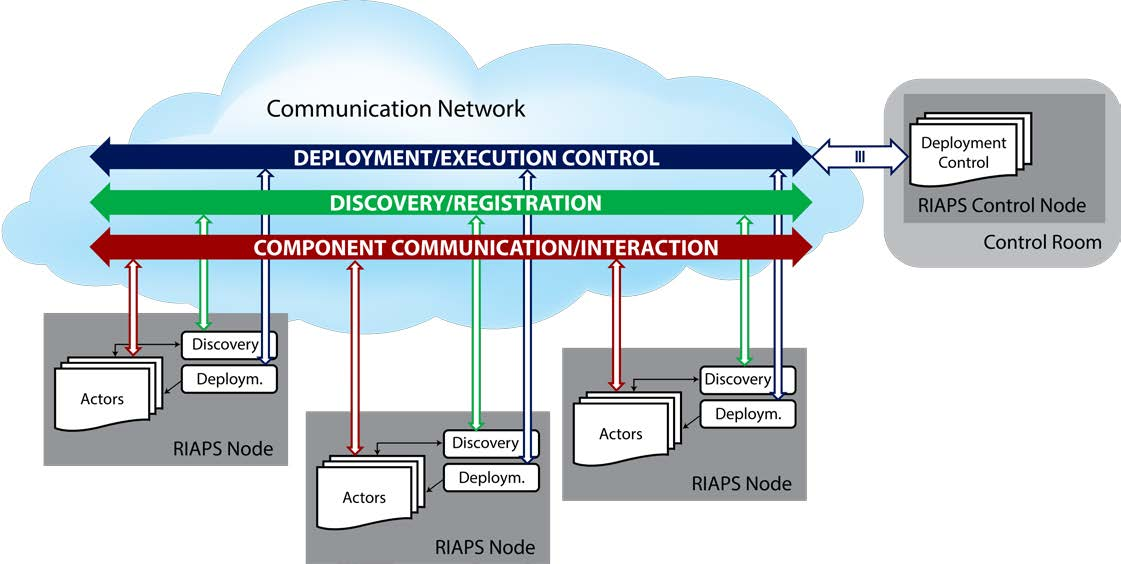
\includegraphics[width=0.48\textwidth]{diagrams/RIAPSBroch_FINALPRINT.jpg}
%   \caption{RIAPS concept.}
% 	\label{fig:concept}
% \end{figure}

In any technical system that relies on embedded computing, the most important ingredient is an ``operating system'' that provides the foundations for all algorithms, isolates the hardware details from the algorithms, and provides essential mechanisms for resource management, fault tolerance, and security. For example, in the work presented in this paper, this framework allows us to disseminate information between the actors. Our extended team has developed a platform called `Resilient Information Architecture Platform for Smart Grid' (RIAPS) \cite{riaps}, where each actor is a composition of several libraries that provide (1) a component model that provides a concurrent model of computation for building distributed real-time applications, (2) a messaging framework for facilitating interactions among actors, (3) a resource-management framework for controlling the use of computational resources, (4) a fault-management framework for detecting and mitigating faults in all layers of the system, (5) a security framework to protect the confidentiality, integrity, and availability of system under cyber-attacks, (6) a fault tolerant time synchronization service,  (7) a discovery framework for establishing the network of interacting actors of an application, and (7) a deployment and management framework for the administration and control of the distributed applications from a control room. 









\subsection{Trading System Architecture}
\label{sec:architecture}


Figure~\ref{fig:components} shows the architecture of the energy trading system. The specific platforms and tools used in our implementation are shown in parentheses and as arrow labels. All components are written in Python and communicate with each other using ZeroMQ, one of the protocols supported by the RIAPS platform. 




\subsection{Providing Privacy}
\label{sec:privacy}

To protect their privacy, prosumers use anonymous addresses when interacting with the blockchain (e.g., posting offers).
By generating new anonymous addresses at random periodically, they can prevent other participants from linking the anonymous addresses to their actual identities~\cite{Laszka17}, thereby keeping their trading activities private. 
However, in contrast with our prior work~\cite{Laszka17}, the addresses used in the workflow described in the next section are not completely anonymous. Since the blockchain-based smart contract has to check feeder-level safety constraints, each anonymous address must be linked to a feeder.
Hence, an anonymous address can hide only the prosumer's identity but not its feeder, which is a manifestation of the trade-off between safety and privacy.\footnote{Actually, participants can remain anonymous among a class of feeders with same number of participants and identical safety constraints.}

However, anonymous addresses pose a further threat to safety.
Since participants can generate anonymous addresses at almost no cost, they could post selling and buying offers for large amounts of energy, without any intention of delivering and without facing any repercussions.
A malicious or faulty participant could easily destabilize the grid with this form of reckless trading.
Consequently, the amount of energy that may be traded by anonymous addresses belonging to a participant must be limited.

Thus, we use the concept of energy assets, initially introduced  in~\cite{Laszka17} and  used in the trading workflow described in the next section.
%\AronC{They were only used but not described in the workflow.}  described in the workflow of above.
%In~\cite{Laszka17}, we introduced \emph{energy assets} to enforce participant-level safety constraints.
An energy asset represents a permission to sell or buy a specific amount of energy in a specific set of  time intervals. 
Each prosumer can ask the DSO to transfer assets to an anonymous address, who can check whether it would be safe to give permission to the participant.
If it would be, then the DSO records this transfer on the blockchain.
Later, when the participant posts an offer from the anonymous address, the smart contract can check whether the address has the assets required for the offer.
Since only the DSO can link the anonymous address to the participant, assets enable enforcing participant-level constraints without violating privacy.


\subsection{Trading Workflow}

Figure~\ref{fig:workflow} illustrates the trading workflow.
For ease of presentation, the figure shows only one prosumer and only a single message of each type.
In practice, a large number of prosumers may interact with the DSO and the smart contract, and each of them may exchange multiple messages.

\newcommand{\msgDesc}[1]{{\footnotesize{\texttt{#1}}}}

The workflow includes the following messages:
\begin{compactitem}
\item 
\msgDesc{withdrawAssets(anonAddress, energy, intervals, amount)}: message sent by a prosumer to the DSO, asking the DSO to transfer energy and/or financial assets from the prosumer's account at the DSO to an anonymous address.
Before sending this message, the prosumer first generates a random anonymous address to protect her privacy.
The message specifies the assets that the prosumer wishes to withdraw (i.e., amount of energy and time intervals) and the anonymous address to which the DSO should transfer them.
Note that the prosumer may send this message long before actually engaging in trading, so the DSO does not have to be online continuously.
\item \msgDesc{failedWithdrawal(anonAddress, msg)}: message sent by the DSO to the prosumer,
notifying the prosumer that the requested assets cannot be withdrawn due to, e.g., energy safety requirements or insufficient funds.
\item \msgDesc{addEnergy(anonAddress, energy, intervals)},\\\msgDesc{addFinancialBalance(anonAddress, amount)}:
smart contract functions called by the DSO (i.e., transactions recorded on the blockchain) in response to the prosumer's request, creating energy and financial assets on the blockchain and transferring them to an anonymous address.
Before recording this transaction, the DSO must first verify that enabling the prosumer to trade these assets does not violate any safety constraints and that the anonymous address is linked to the correct feeder.
%The call specifies the assets and the anonymous address to which they are transferred. 
\item \msgDesc{AssetAdded(anonAddress, energy, intervals)},\\\msgDesc{FinancialAdded(anonAddress, amount)}: broadcast messages emitted by the smart contract (i.e., events logged on the blockchain),
notifying the prosumer that the requested assets have been transferred to the anonymous address.
\item \msgDesc{postOffer(energy, intervals, price)}: smart-contract function called by a prosumer (from its anonymous address), publicly posting an energy bid or ask.
%If the prosumer is interested in buying energy, then it posts an energy bid, which specifies an energy consumption asset and a price.
%If the prosumer is interested in selling, then it posts an energy ask, which specifies an energy production asset and a price.
%In both cases, the transaction must be cryptographically signed by the private key of the address, and it locks the assets until the offer is accepted or rescinded.
\item \msgDesc{OfferPosted(offerID, energy, intervals, price)}:
message broadcast by the smart contract, notifying solvers that an offer was posted.
\item \msgDesc{submitSolution(powers, prices)}:
smart-contract function called by a solver,
submitting a new solution for the energy trading problem. %If the offer was an energy bid, then the other prosumer has to provide an energy production assets;
%if the offer was an energy ask, then the other prosumer has to provide both energy consumption and financial assets.
%In both cases, the transaction must be cryptographically signed by the private key of the other prosumer's anonymous address.
%If there is an overlap between the time intervals of the offered asset, and the asset provided by the other prosumer, then the intersecting parts of the assets are exchanged and the non-overlapping parts are returned to their original owners.
%Similarly, based on the price and exchanged energy assets, a part of the financial asset is transferred to the seller, while the rest is returned to the seller. 
\item \msgDesc{SolutionFinalized(powers, prices)}:
message broadcast by the smart contract,
notifying both prosumers and solvers of energy trades that have been finalized. %that its offer has been accepted, and the assets have been exchanged.
\item \msgDesc{depositEnergy(energy, intervals)},\\\msgDesc{depositFinancial(amount)}:
smart-contract functions called by a prosumer,
depositing energy and financial assets to the prosumer's account.
%The transaction specifies the assets, and it must be cryptographically signed by the anonymous address that owns them.
Note that to protect privacy, the calls do not specify the prosumer, so the DSO has to keep track of which prosumer has used which anonymous address.
\item \msgDesc{EnergyDeposited(anonAddress, energy, intervals)},\\\msgDesc{FinancialDeposited(anonAddress, amount)}:
messages broadcast by the smart contract,
notifying the DSO that assets have been deposited from anonymous address, which triggers the transfer of these assets to the prosumer's account at the DSO.
\end{compactitem}

\subsection{Implementation Considerations}
\label{sec:implementation}

\subsubsection{Parameters} The system of prosumers, solvers, DSO, and smart contract operates mostly asynchronously. The only synchronous communication  occurs between prosumers and the DSO. They all operate as  independent processes running on remote nodes, with their own time bases. In particular, the solver can operate as a periodic process (with a period $\Delta_s$), waiting on information from the smart contract about all the offers that have been posted in the prior period. The prosumers  can also operate as periodic processes, submitting their offers and bids to the smart contract.  In practice, prosumers will be synchronized with real wall-clock time, making their bids and asks known for future intervals, depending upon the time at which they post their bids/asks and how far in the future  they can predict their usage or operation. We make  their prediction window $L$ a parameter of the system. The value of this parameter is at least $2$, because prosumers have to  make a bid/ask for at least the next interval (we count the current interval in $L$). A larger value of this prediction window will increase the risk of uncertainty for the prosumer, since they are expected to be able to fulfill their bid or ask.\footnote{The size of the prediction window is part of the prosumer strategy, which is not explored in this paper as our focus is on the implementation of the TMP.} Additionally, during our experiments, we can simulate $\Delta$ as $\hat{\Delta}$ to speed up the process.\footnote{Note that this is the amount of real time passed in the simulation before proceeding to the next interval. This allows us to speed things up for the experiment, since running the system slower would just be easier.} These parameters are described in Table \ref{tab:symbols}.

\subsubsection{Speed and Synchronization Considerations}
A relevant problem for TMP is deciding how fast it can run and ensuring that trades for the next interval can clear before the $T_{clear}$ parameter, which has a minimum bound of $1$.
In our system, regular network communication mechanisms are assumed to be fast. However, the communication with the smart contract is limited by the block mining rate, and we need multiple messages exchanged in each interval (see Figure~\ref{fig:workflow}), so the miners need to work fast enough to mine a few blocks in each time interval. In a closed environment, this can be achieved by reducing the difficulty of the cryptographic puzzle solved for proof-of-work consensus. In our system, as shown in the next section, we are able to clear transactions much faster than one time interval. 
For larger systems, the proof-of-work consensus may be replaced by, e.g., proof-of-stake, for scalability.

Another problem is the synchronization between the different agents. The runtime platform of RIAPS provides us with high-precision time synchronization \cite{riaps2}. However, even if we only have NTP as the synchronization mechanism, we can operate the system correctly. This is because intervals in practice are relatively (i.e.,  compared to typical communication delays) long (e.g., 15 minutes). Additionally, the smart contract can ensure that the system always proceeds to the next time interval (however, the accuracy of this is limited by the mining rate, see previous paragraph). Additionally, our system can  tolerate or discard out-of-order and late messages due to the event chronology implemented in the blockchain platform. In practice, however, prosumers should try to post their offers early within a time interval, so that solvers will include them in the solution for the current time interval. On the other hand, solvers should wait some time before starting to work, so that they can collect all (or at least most) of the offers posted in the interval.

% \Aron{Talk about timing issues in smart contracts!}

% \color{red}
% Ideas:
% \begin{itemize}
% \item communication over the blockchain is limited by the block mining rate, and we need multiple messages exchanged in each interval, so the miners need to work fast enough to mine a few blocks in each time interval
% \item no time synchronization is necessary since 1) intervals in practice are relatively (i.e.,  compared to typical communication delays) long (e.g., 15 minutes) 2) smart contract can ensure that the system always proceeds to the next time interval (however, the accuracy of this is also limited by the mining rate, see previous point) 3) our system can tolerate or discard out-of-order and late messages\AbhishekC{Can we address what will happen if there are multiple miners.}
% \item in practice, prosumers should try to post their offers early within a time interval, so the solver can include them in the solution for the current time interval; on the other hand, solvers should wait some time before starting to work so that they have all (or at least most) of the offers posted in the interval
% \end{itemize}
% \color{black}


% % !TeX root = ICCPS18.tex
% \subsection{Implementation}

% \begin{figure}
% 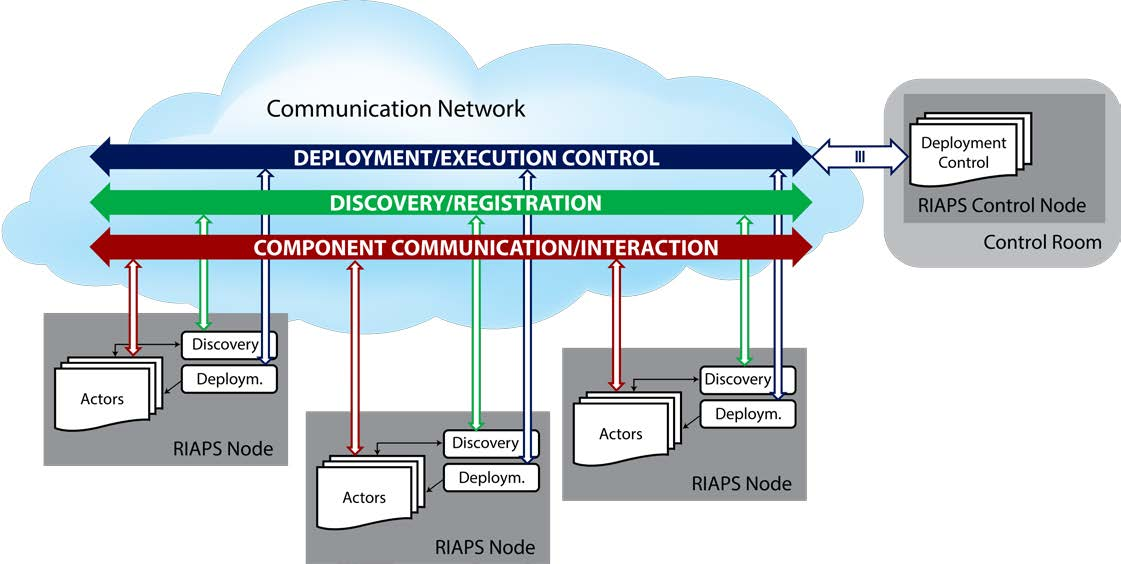
\includegraphics[width=0.48\textwidth]{diagrams/RIAPSBroch_FINALPRINT.jpg}
%   \caption{RIAPS concept.}
% 	\label{fig:concept}
% \end{figure}

% \AronC{This is the only ``subsubsection'' within this subsection.}
% \Abhishek{Aron- the smart contract discussion and the wrapper implementation discussion should go into this section}

% \subsubsection{Background}
% In any technical system that relies on embedded computing, the most important ingredient is an ``operating system'' that provides the foundations for all algorithms, isolates the hardware details from the algorithms, and provides essential mechanisms for resource management, fault tolerance, and security. For example, in the work presented in this paper, this framework allows us to disseminate information between the actors. This platform called `Resilient Information Architecture Platform for Smart Grid' (RIAPS) \cite{riaps} has been developed by our extended team, where each actor is a composition of several libraries that provide (1) a component model that provides a concurrent model of computation for building distributed real-time applications, (2) a messaging framework for facilitating interactions among actors, (3) a resource-management framework for controlling the use of computational resources, (4) a fault-management framework for detecting and mitigating faults in all layers of the system, (5) a security framework to protect the confidentiality, integrity, and availability of system under cyber-attacks, (6) a fault tolerant time synchronization service,  (7) a discovery framework for establishing the network of interacting actors of an application, and (7) a deployment and management framework for the administration and control of the distributed applications from a control room. 


% \subsubsection{Smart Contract}


% \subsubsection{SmartHomeTrader}


% \subsubsection{Solver}


% \Abhishek{Aron we need to describe the implementation architecture.}

% \begin{itemize}
% \item communication is implemented via ZeroMQ
% \item timesynchronization is implemented via PTP and NTP 
% \item Resource discovery if required can be provided by RIAPS. Not required for this experiment.
% \begin{itemize}
% \item The basic implementation pattern is using wrappers to connect to blockchain. Why is this important.
% \item What does the prosumer script do
% \item run one geth client per prosumer
% \item multiple miner nodes can run.
% \item The full architecture includes DSO script, 
% \item Evaluation - Timing and Network Overhead
% \end{itemize}
% \end{itemize}

% !TeX root = ICCPS18.tex
\section{Experimental Evaluation and Discussions}
\label{sec:results}

We consider a collection of load traces recorded by Siemens from a microgrid in Germany, containing $102$ homes across $11$ feeders ($5$ producers and $97$ consumers). %Table \ref{tab:prosumers}
Figure~\ref{fig:feeder} describes the feeder structure, the number of participants per feeder, and  the feeder safety limits. We use $\Delta =15$ minute intervals, resulting in a total of $96$ intervals across the whole day.   Figure~\ref{fig:profile} shows the total production and consumption across this microgrid. The horizontal axis shows the starting time for each of the $96$ intervals. 
\AronC{I added this to address the lack of prices in our }
Since the dataset does not include prices, we assume reservation prices to be uniform in our experiments, and focus on studying the amount of energy traded and the performance of the system.

As one of our primary contributions in this work is the ability to specify multiple time intervals for  selling offers, we extended the trace that was collected by Siemens to allow each producer to have a battery with a total capacity of $90$ kWh. With a battery, a producer can take the energy produced in  a time interval and decide to make it available in future time intervals.
Note that the resulting offers always span a contiguous set of time intervals, so they can be specified by their starting time and length. 
Figure \ref{fig:batteryEffect} shows these intervals for one particular producer. The producers charge their batteries only when the total consumption is less than the total production, which happens just after 12:00 PM, see Figure~\ref{fig:profile}.


% !TeX root = ICCPS18.tex
  \definecolor{blueLine}{RGB}{57,106,177}
\definecolor{blueFill}{RGB}{114,147,203}
\definecolor{redLine}{RGB}{204,37,41}
\definecolor{greenline}{RGB}{0,250,0}
\definecolor{blackLine}{RGB}{0,0,0}
\definecolor{goldLine}{RGB}{160,82,45}
 
     \begin{figure}[t]
 \centering
\resizebox{0.45\textwidth}{!}{%
 \begin{tikzpicture}[rotate=270,font=\tiny,
   oc/.style={fill=black,rectangle,minimum size=0.01cm,font=\tiny},
     feeder/.style={fill=brown,rectangle,minimum size=0.005cm,font=\tiny},
   Producer/.style={fill=green,circle,minimum size=0.01cm},
     Consumer/.style={fill=red,circle,minimum size=0.01cm},
   Connection/.style={<->, >=stealth, shorten <=0.05cm, shorten >=0.05cm}]
 \draw node[oc] (oc1) at (-5,0){};
 \draw node[oc] (oc2) at (-4,0){};
 \draw node[oc] (oc3) at (-3,0){};
 \draw node[oc] (oc4)  at (-2,0){};
 \draw node[oc](oc5)  at (-1,0){};
 \draw node[oc] (oc6)  at (0,0){};
 \draw node[oc] (oc7) at (1,0){};
 \draw node[oc] (oc8)  at (2,0){};
 \draw node[oc] (oc9) at (3,0){};
 \draw node[oc] (oc10) at (4,0){};
 \draw node[oc] (oc11) at (5,0){};

 \draw node[feeder] (feeder1) at (-5,-1){};
 \draw node[feeder] (feeder2) at (-4,-1){};
 \draw node[feeder] (feeder3) at (-3,-1){};
 \draw node[feeder] (feeder4)  at (-2,-1){};
 \draw node[feeder](feeder5)  at (-1,-1){};
 \draw node[feeder] (feeder6)  at (0,-1){};
 \draw node[feeder] (feeder7) at (1,-1){};
 \draw node[feeder] (feeder8)  at (2,-1){};
 \draw node[feeder] (feeder9) at (3,-1){};
 \draw node[feeder] (feeder10) at (4,-1){};
 \draw node[feeder] (feeder11) at (5,-1){};

 \draw [Connection] (feeder1) to (feeder2);
 \draw [Connection] (feeder2) to (feeder3);
 \draw [Connection] (feeder3) to (feeder4);
 \draw [Connection] (feeder4) to (feeder5);
 \draw [Connection] (feeder5) to (feeder6);
 \draw [Connection] (feeder6) to (feeder7);
 \draw [Connection] (feeder7) to (feeder8);
 \draw [Connection] (feeder8) to (feeder9);
 \draw [Connection] (feeder9) to (feeder10);
 \draw [Connection] (feeder10) to (feeder11);

\draw [Connection] (feeder1) to (oc1);
\draw [Connection] (feeder2) to (oc2);
\draw [Connection] (feeder3) to (oc3);
\draw [Connection] (feeder4) to (oc4);
\draw [Connection] (feeder5) to (oc5);
\draw [Connection] (feeder6) to (oc6);
\draw [Connection] (feeder7) to (oc7);
\draw [Connection] (feeder8) to (oc8);
\draw [Connection] (feeder9) to (oc9);
\draw [Connection] (feeder10) to (oc10);
\draw [Connection] (feeder11) to (oc11);


 \foreach \pos in {1,2} {
   \node [Producer] (p10\pos)at (-5,\pos) {};
 }

 \foreach \pos in {3,4,5,6,7,8,9} {
   \node [Consumer] (c10\pos)at (-5,\pos) {};
 }

 \foreach \pos in {1,2,3,4,5,6,7,8,9,10,11,12,13,14,15,16,17} {
   \node [Consumer] (c20\pos)at (-4,\pos) {};
 }

 \foreach \pos in {1,2,3,4,5} {
   \node [Consumer] (c30\pos)at (-3,\pos) {};
 }


 \foreach \pos in {1,2,3,4,5,6,7,8,9,10,11,12,13} {
   \node [Consumer] (c40\pos)at (-2,\pos) {};
 }


 \foreach \pos in {1,2,3,4,5,6,7,8} {
   \node [Consumer] (c50\pos)at (-1,\pos) {};
 }


 \foreach \pos in {1} {
   \node [Consumer] (c60\pos)at (0,\pos) {};
 }


 \foreach \pos in {1} {
   \node [Producer] (p70\pos)at (1,\pos) {};
 }


 \foreach \pos in {2,3,4,5,6,7,8,9,10,11} {
   \node [Consumer] (c70\pos)at (1,\pos) {};
 }


 \foreach \pos in {17} {
   \node [Producer] (p80\pos)at (2,\pos) {};
 }

 \foreach \pos in {1,2,3,4,5,6,7,8,9,10,11,12,13,14,15,16} {
   \node [Consumer] (c80\pos)at (2,\pos) {};
 }

 \foreach \pos in {1,2,3,4,5} {
   \node [Consumer] (c90\pos)at (3,\pos) {};
 }

 \foreach \pos in {11} {
   \node [Producer] (p100\pos)at (4,\pos) {};
 }

 \foreach \pos in {1,2,3,4,5,6,7,8,9,10,12,13} {
   \node [Consumer] (c100\pos)at (4,\pos) {};
 }

 \foreach \pos in {1,2,3,4,5} {
   \node [Consumer] (c110\pos)at (5,\pos) {};
 }


 \draw [Connection] (oc1) to (p101);
 \draw [Connection] (p101) to (p102);
 \draw [Connection] (p102) to (c103);
 \draw [Connection] (c103) to (c104);
 \draw [Connection] (c104) to (c105);
 \draw [Connection] (c105) to (c106);
 \draw [Connection] (c106) to (c107);
 \draw [Connection] (c107) to (c108);
 \draw [Connection] (c108) to (c109);
 
\draw [Connection] (oc2) to (c201);
\draw [Connection] (c201) to (c202);
\draw [Connection] (c202) to (c203);
\draw [Connection] (c203) to (c204);
\draw [Connection] (c204) to (c205);
\draw [Connection] (c205) to (c206);
\draw [Connection] (c206) to (c207);
\draw [Connection] (c207) to (c208);
\draw [Connection] (c208) to (c209);
\draw [Connection] (c209) to (c2010);
\draw [Connection] (c2010) to (c2011);
\draw [Connection] (c2011) to (c2012);
\draw [Connection] (c2012) to (c2013);
\draw [Connection] (c2013) to (c2014);
\draw [Connection] (c2014) to (c2015);
\draw [Connection] (c2015) to (c2016);
\draw [Connection] (c2016) to (c2017);

\draw [Connection] (oc3) to (c301);
\draw [Connection] (c301) to (c302);
\draw [Connection] (c302) to (c303);
\draw [Connection] (c303) to (c304);
\draw [Connection] (c304) to (c305);

\draw [Connection] (oc4) to (c401);
\draw [Connection] (c401) to (c402);
\draw [Connection] (c402) to (c403);
\draw [Connection] (c403) to (c404);
\draw [Connection] (c404) to (c405);
\draw [Connection] (c405) to (c406);
\draw [Connection] (c406) to (c407);
\draw [Connection] (c407) to (c408);
\draw [Connection] (c408) to (c409);
\draw [Connection] (c409) to (c4010);
\draw [Connection] (c4010) to (c4011);
\draw [Connection] (c4011) to (c4012);
\draw [Connection] (c4012) to (c4013);

\draw [Connection] (oc5) to (c501);
\draw [Connection] (c501) to (c502);
\draw [Connection] (c502) to (c503);
\draw [Connection] (c503) to (c504);
\draw [Connection] (c504) to (c505);
\draw [Connection] (c505) to (c506);
\draw [Connection] (c506) to (c507);
\draw [Connection] (c507) to (c508);

\draw [Connection] (oc6) to (c601);

\draw [Connection] (oc7) to (p701);
\draw [Connection] (p701) to (c702);
\draw [Connection] (c702) to (c703);
\draw [Connection] (c703) to (c704);
\draw [Connection] (c704) to (c705);
\draw [Connection] (c705) to (c706);
\draw [Connection] (c706) to (c707);
\draw [Connection] (c707) to (c708);
\draw [Connection] (c708) to (c709);
\draw [Connection] (c709) to (c7010);
\draw [Connection] (c7010) to (c7011);

\draw [Connection] (oc8) to (c801);
\draw [Connection] (c801) to (c802);
\draw [Connection] (c802) to (c803);
\draw [Connection] (c803) to (c804);
\draw [Connection] (c804) to (c805);
\draw [Connection] (c805) to (c806);
\draw [Connection] (c806) to (c807);
\draw [Connection] (c807) to (c808);
\draw [Connection] (c808) to (c809);
\draw [Connection] (c809) to (c8010);
\draw [Connection] (c8010) to (c8011);
\draw [Connection] (c8011) to (c8012);
\draw [Connection] (c8012) to (c8013);
\draw [Connection] (c8013) to (c8014);
\draw [Connection] (c8014) to (c8015);
\draw [Connection] (c8015) to (c8016);
\draw [Connection] (c8016) to (p8017);

\draw [Connection] (oc9) to (c901);
\draw [Connection] (c901) to (c902);
\draw [Connection] (c902) to (c903);
\draw [Connection] (c903) to (c904);
\draw [Connection] (c904) to (c905);

\draw [Connection] (oc10) to (c1001);
\draw [Connection] (c1001) to (c1002);
\draw [Connection] (c1002) to (c1003);
\draw [Connection] (c1003) to (c1004);
\draw [Connection] (c1004) to (c1005);
\draw [Connection] (c1005) to (c1006);
\draw [Connection] (c1006) to (c1007);
\draw [Connection] (c1007) to (c1008);
\draw [Connection] (c1008) to (c1009);
\draw [Connection] (c1009) to (c10010);
\draw [Connection] (c10010) to (p10011);
\draw [Connection] (p10011) to (c10012);
\draw [Connection] (c10012) to (c10013);


\draw [Connection] (oc11) to (c1101);
\draw [Connection] (c1101) to (c1102);
\draw [Connection] (c1102) to (c1103);
\draw [Connection] (c1103) to (c1104);

 \end{tikzpicture}
 }
 \caption{Feeder diagram. Brown nodes are feeder junctions, numbered 1 to 11 from top to bottom.  Black nodes are the overcurrent relays, which ensure that the total power flowing in and out of the feeder is below 20 kW. The green nodes are the junction points for the producers ($5$), and the red nodes are junction points for the consumers ($97$). There are $102$ prosumers in total.}
 \label{fig:feeder}
 \end{figure}







\begin{figure}[ht]
\begin{tikzpicture}
\begin{axis}[
  font=\footnotesize,
  width=\columnwidth,
  height=0.61\columnwidth,
  ymin=2865,
  ymax=2975,
  ytick={2875,2900,2925,2950},
  xtick={2,3,5,7,10,13},
  legend pos=north west,
  xlabel={Prosumer prediction window [time intervals]},
  ylabel={Total energy traded [kWh]},
grid=both,
    grid style={line width=.1pt, draw=gray!10},
    major grid style={line width=.2pt,draw=gray!50},
]
\addplot[mark=o, color=blueLine, only marks, thick] table[x=predictionWindow, y=withoutBattery, comment chars={\%}, col sep=comma] {diagrams/total-energy-traded.csv};
\addlegendentry{without battery};
\addplot[mark=+, color=redLine, only marks, thick] table[x=predictionWindow, y=withBattery, comment chars={\%}, col sep=comma] {diagrams/total-energy-traded.csv};
\addlegendentry{with battery};
\end{axis}
\end{tikzpicture}
\caption{Total amount of energy traded in the entire microgrid with and without batteries, for various prediction window lengths.}
\label{fig:multihorizon}
\end{figure}


\begin{figure}[t]
	\centering
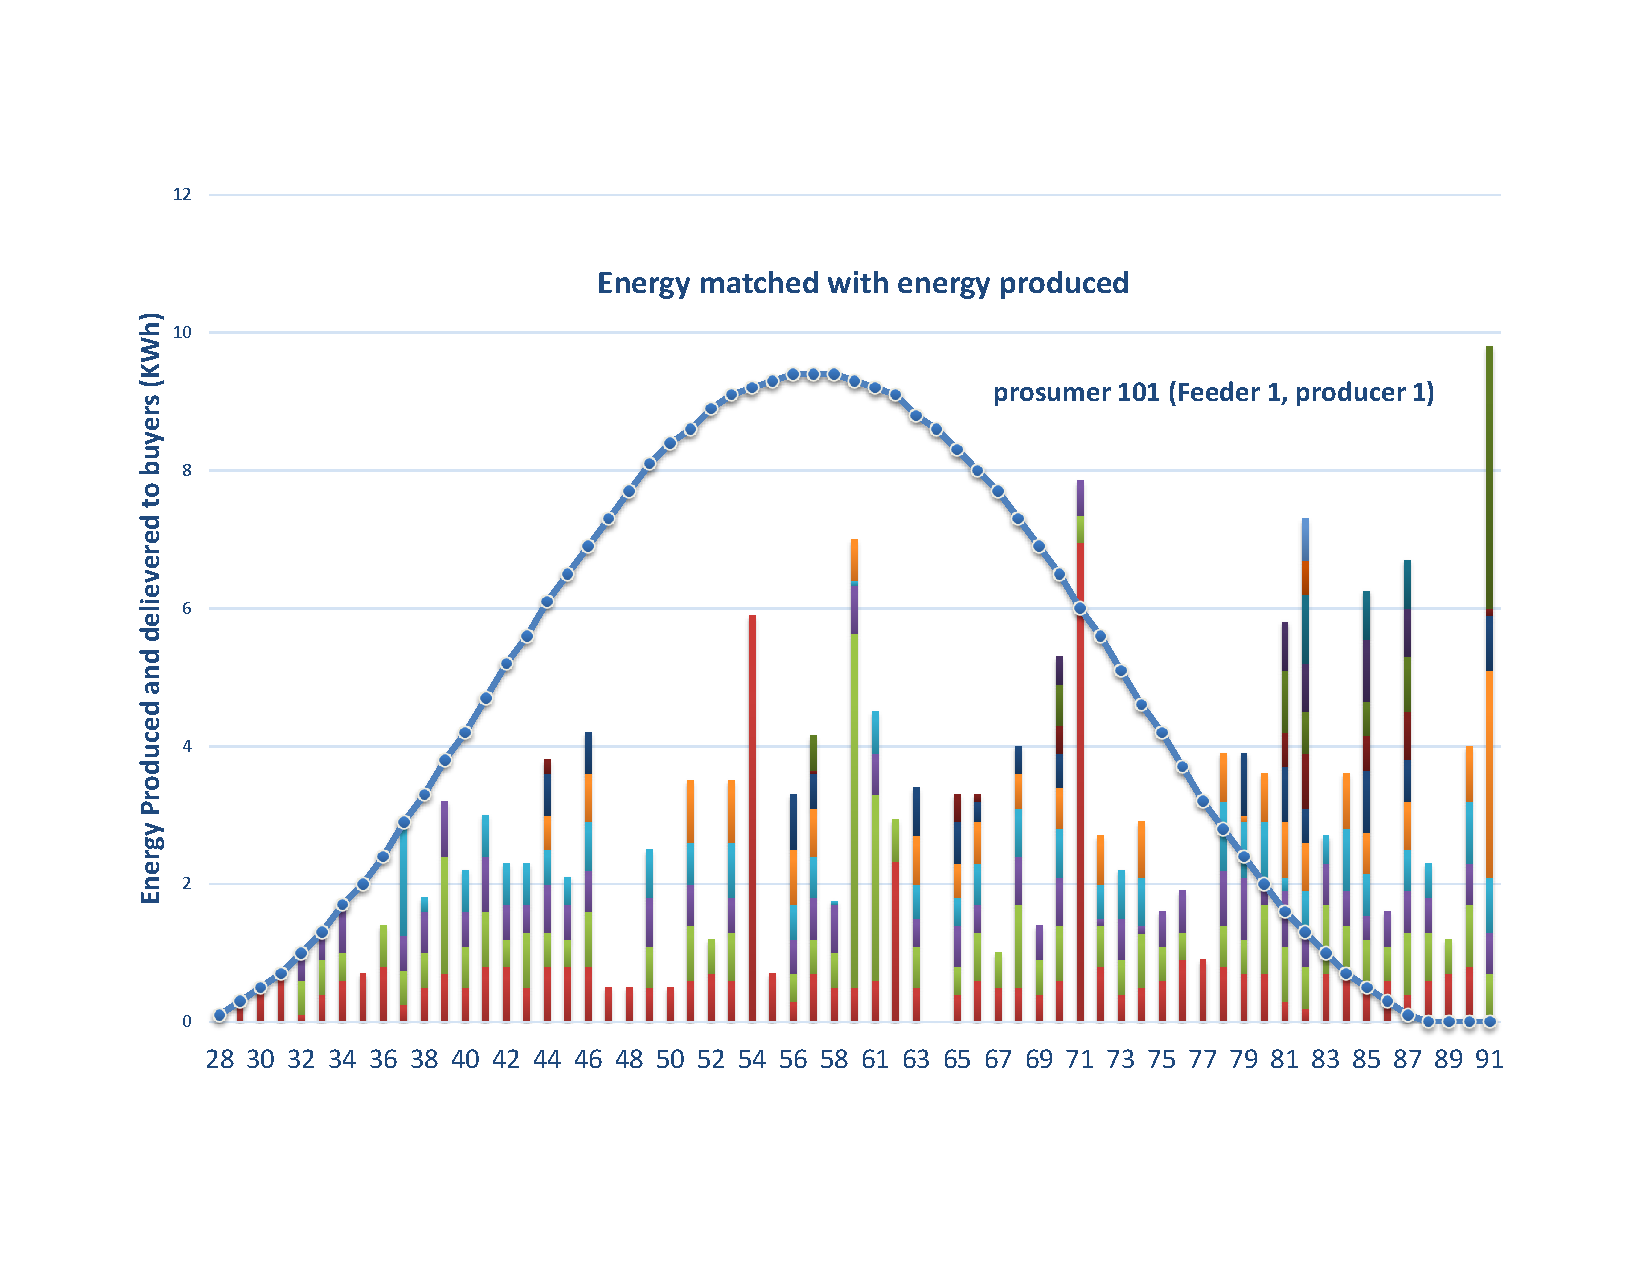
\includegraphics[width=1\columnwidth]{diagrams/prosumer101.pdf}
	\caption{Energy generated in each interval (blue line) and energy traded to a set of consumers in each interval (vertical bars) for the first prosumer of the first feeder (Test case C). The stacked colors show the different consumers that were matched with the prosumer in each interval (note that the same color across multiple intervals does not necessarily mean the same consumer). When the energy traded exceeds the generation, the excess is drawn from the battery.}
	\label{fig:allocate1NRG}
\end{figure}

\begin{figure}[htb]
	\centering
    \begin{tikzpicture}
    	\begin{axis}[
	width=\columnwidth,
	height=0.5\columnwidth,
	bar width=0.04\textwidth,
    font=\footnotesize,
    grid=both,
    grid style={line width=.1pt, draw=gray!10},
    major grid style={line width=.2pt,draw=gray!50},
	ybar,
	ytick={0, 5, 10, 15, 20},
	%yticklabels={40, 60, 90, 135},
	xlabel style={align=center},
	xlabel={Real time [seconds]},
	ylabel={Number of Offers},
	symbolic x coords={0,1,2,3,4,5},
	xticklabels={{[11, 23]}, {(23, 35]}, {(35, 47]}, {(47, 59]}, {(59, 71]}, {(71, 84]}},
	xtick=data,
	ylabel style={align=center},
	]
\addplot[fill=blueFill] coordinates { 
		(0, 20)
		(1, 20)
		(2, 12)
		(3, 5)
		(4, 1)
		(5, 1)
	};
	\end{axis}
\end{tikzpicture}
%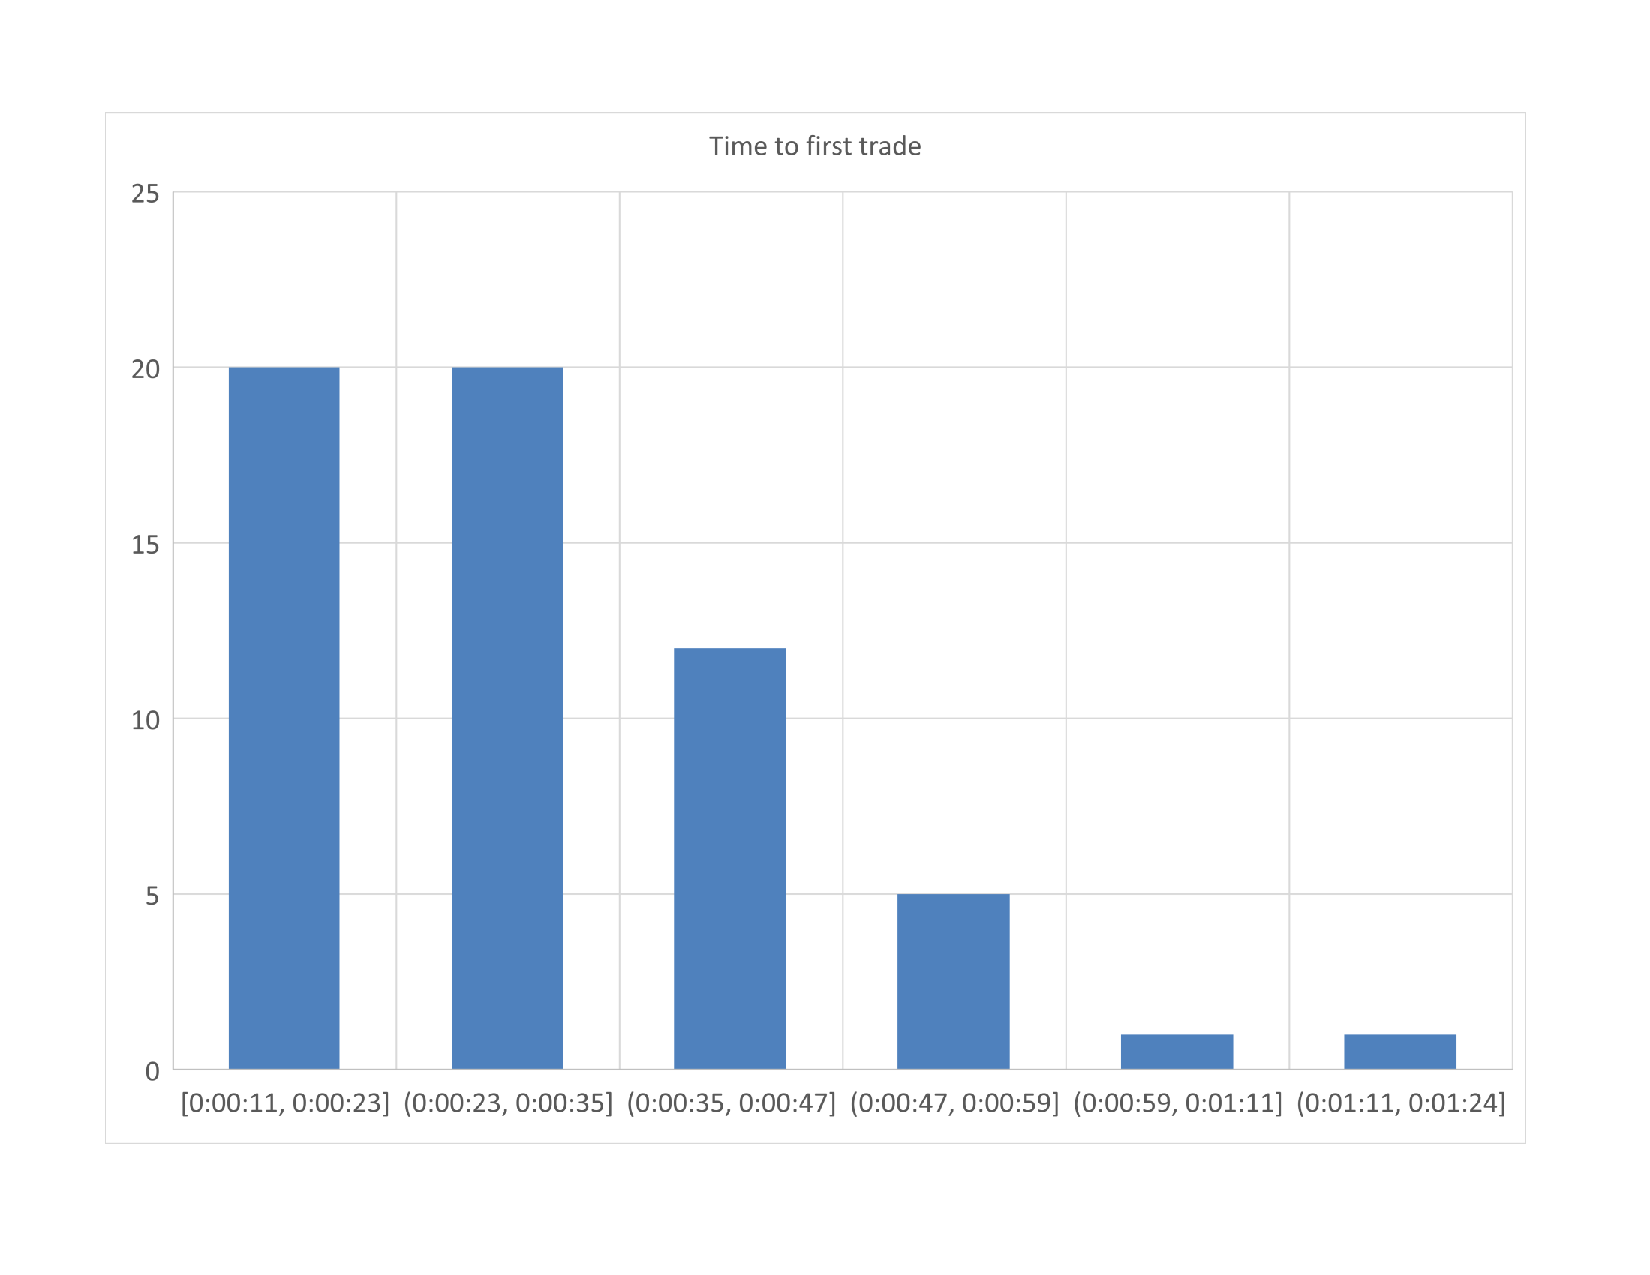
\includegraphics[width=1\columnwidth]{diagrams/timechart.pdf}
	\caption{Real time in seconds between posting an offer and recording a trade that includes the offer (Test case C). This time includes the communication delay, the time to mine the blockchain, and the running time required to find a solution. Since the solver runs periodically and receives offers asynchronously, there might be a few runs before a suitable match is found.}
	\label{fig:time}
\end{figure}


%\textcolor{red}{Table ... describes our data conversion rules.}







\subsection{Test Bed}
The hardware test bed is a cluster of 31 BeagleBone Black~\footnote{https://beagleboard.org/black} (BBB)  single-board computers (see Figure~\ref{fig:testbed_architecture}) acting as participants in the energy trading system. The BBBs are set up as light clients because they are resource constrained and therefore are not suitable for mining or acting as solvers. This means that they can safely access the blockchain but do not participate in the consensus process.  In the dataset provided by Siemens, there are 95 consumers and 7 producers of power,  see Figure \ref{fig:components}. These participants are divided between the BBBs in the cluster. The  PlaTIBART (Platform for Transactive IoT Blockchain Applications with Repeatable Testing platform) \cite{platibart}  platform provided us with the necessary devops support.

The block mining is provided by external hardware, locally or in a cloud server. We had a single miner instance that was responsible for maintaining the blockchain, and a single solver instance that used CPLEX \cite{cplex2009v12} to solve the energy trading problem. This setup can be easily scaled to add more miners and solvers if there are enough computational resources available. The communication between the components was implemented using ZeroMQ, which is one of the communication protocols available in RIAPS. 

%To evaluate our approach, we use a decentralized blockchain testbed that has been established in our lab. The  PlaTIBART (Platform for Transactive IoT Blockchain Applications with Repeatable Testing platform) \cite{platibart}  platform provided us with the necessary devops support to start the trading processes for all $102$ homes in the system, see Figure \ref{fig:components}. 








\subsection{Experiments}
Table~\ref{table:test-parameters} describes the specifics of the four categories of tests that we ran. The tests vary the different implementation parameters (see Table \ref{tab:symbols} and Section~\ref{sec:implementation}). This allows us to study how changing these parameters affects the total amount of energy traded. 

Figure \ref{fig:multihorizon} shows the total energy traded for different tests. We varied the prediction window ($L$) for the participants from $2$ to $13$. That is, in each interval, the participants submitted offers starting from the next $1$ to $12$ intervals (current interval is always counted in the prediction window). The experiment simulated the whole day from the first interval starting at 0:00 (12:00 AM) to the $95^{th}$ interval ending at 23:59 (11:59 PM). % in the next night.
%
As expected, increasing the prediction window without batteries has no effect on the total amount energy traded. This is because any production must be dispatched within one time interval, so the solver cannot optimize energy usage across multiple intervals even if future offers are available. % So, the solver can never use the energy from a previous interval in a producer to provide energy to a consumer in a subsequent interval.

However, this is possible if there are batteries in the system. With batteries, the amount of energy traded increases as we allow the solver to match offers across multiple time intervals at once. Trading increases with the prediction window because of the increased analysis space available to the solver.
Figure~\ref{fig:profile} shows the  per interval trades for three of these cases (A, C, and D): without battery, with battery and $L=5$, as well as with battery and $L=13$.  

Figure \ref{fig:allocate1NRG} shows the energy matched per interval in test case~C for the first prosumer of the first feeder. Figure \ref{fig:time} shows a histogram of the time between posting an offer and recording a trade on the blockchain that includes the offer (also in test case C). The time length was always less than $\hat{\Delta}$, which was $120$ seconds (see Table \ref{table:test-parameters}).
\ifShowLog
Figure \ref{fig:log} shows an extract of raw log messages from the system that were used to produce this chart.
\fi

\ifShowLog
\definecolor{keywords}{HTML}{8A4A0B}
\definecolor{background}{HTML}{EEEEEE}
\definecolor{comments}{HTML}{868686}

\lstdefinelanguage{log}{
 morekeywords={ prosumer,  INFO, Postingoffers, SellingOfferPosted, TradeAdded, solutionID, time, objective, buyerID, power, energy, sellerID},
 keywordstyle=\color{keywords},
 basicstyle=\scriptsize\ttfamily,
 morecomment=[l]{//}, 
 morecomment=[s]{/*}{*/}, 
 morestring=[b]",
 basicstyle=\scriptsize\ttfamily,%
 commentstyle=\color{comments}\ttfamily,
numbers=none,
    numberstyle=\scriptsize,
    stepnumber=1,
    numbersep=8pt,
breaklines=true,
    frame=tb,
 tabsize=4}
 
 \begin{figure}
 \begin{lstlisting}[language=log,numbers=none]
2017-10-12 03:27:05,122 / prosumer 101 / INFO: Posting offers for interval 28...
...
2017-10-12 03:27:05,123 / prosumer 101 / INFO: postSellingOffer(101, 28, 28, 100)
...
2017-10-12 03:27:19,973 / prosumer 101 / INFO: SellingOfferPosted({'endTime': 28, 'ID': 6, 'startTime': 28, 'prosumer': 101, 'energy': 100}).
...
2017-10-12 03:27:38,131 / prosumer 101 / INFO: TradeAdded({'solutionID': 1, 'time': 28, 'objective': 5400, 'buyerID': 133, 'energy': 100, 'sellerID': 6}).
...
 \end{lstlisting}
 \caption{Example log output from prosumer 101. The \texttt{postSellingOffer} call happens when the prosumer posts the selling offer. At the same time, there are prosumers who have posted the buying offer. The smart contract records the offer and the event \texttt{SellingOfferPosted} is generated. We see the \texttt{TradeAdded} event when the solution has been generated by the solver and certified by the smart contract. The objective is the total energy traded. All values have been scaled by $1000$ to account for the problem that the current Ethereum smart contract cannot handle floating-point numbers. Thus the actual objective value is $5.4$ kWh.\textcolor{red}{take out this figure if space is needed}}
 \label{fig:log}
 \end{figure}
\fi

\subsection{Discussion}

\Abhishek{The discussion should include reinforcement about the privacy aspect. it should also explain how using blockchains enables us to handle malicious actors. we should discuss why decentralization is better for resilience.}

\Abhishek{Describe the lessons learned as an itemized list}

We conclude our evaluation by providing a brief discussion of how our platform satisfies the requirements listed in Section~\ref{sec:requirements} (see Table~\ref{tab:discussion} for a summary).
First, the communication architecture is provided by Ethereum and our middleware RIAPS.
Our performance results in Figure~\ref{fig:time} demonstrate that our platform can process and match trades much faster than what would typically be required in practice (Section~\ref{sec:implementation}).
Second, we enforce feeder-level operational safety and stability constraints on trading using a blockchain-based smart contract (Section~\ref{sec:hybridSolver}).
These are in addition to the prosumer-level constraints enforced by tracking energy assets~(Section~\ref{sec:privacy}, \cite{Laszka17}).
Third, we ensure market efficiency and security by enabling the smart contract to validate and evaluate the trading solutions that it receives (Section~\ref{sec:hybridSolver}).
Finally, we provide privacy for prosumers by allowing them to hide their identity using anonymous addresses (Section~\ref{sec:privacy} and~\cite{Laszka17}). However, prosumers are required to reveal which feeder they belong to in order to enable enforcing feeder-level safety constraints.

\begin{table}[h]
\caption{Requirements and Proposed Solutions}
\label{tab:discussion}
\centering
\setlength{\tabcolsep}{0.3em}
\renewcommand*{\arraystretch}{1.3}
\begin{tabular}{|p{2.6cm}|p{5.75cm}|}
\hline
Requirement & Proposed Solution \\
\hline
\hline
Communication Fabric & RIAPS~\cite{riaps} and Ethereum \\
\hline
Operational Safety and Stability & feeder-level constraints modeled in the energy trading problem and enforced by the smart contract (Section~\ref{sec:hybridSolver}); prosumer-level constraints enforced by energy asset tracking~(Section~\ref{sec:privacy}, \cite{Laszka17}) \\
\hline
Market Efficiency and Security & objective modeled in the energy trading problem and enforced by the smart contract (Section~\ref{sec:hybridSolver})\\
\hline
Privacy & anonymous addresses~(Section~\ref{sec:privacy}, \cite{Laszka17}) \\
\hline
\end{tabular}
\end{table}


During the design and evaluation of our platform, one of the main challenges was the conflict between safety, privacy, and efficiency.
For example, the enforcement of feeder-level safety constraints required prosumers to reveal their feeder during trading, instead of staying completely anonymous.
Further, feeder-level safety constraints can also prevent meeting energy demand with local supply, even if there is surplus production in the microgrid (Figure~\ref{fig:profile}).

\section{Conclusion}
\label{sec:concl}


\bibliographystyle{IEEEtran}
\bibliography{references} 

\clearpage
%\clearpage
\section{Draft}

%\Karla{An idea: Carry out a two-stage market. First at the feeder level: match as much supply and demand at the feeder. Second: take what is left over and run a second matching at the inter-feeder level. Advantages: (1) satisfying capacity constraints could be simplified. (2) aggregating residual supply/demand and running a separate inter-feeder market could help make privacy easier? (3) matching itself might be simpler?}

%\Aron{Regarding aggregation at the feeder level: This might give us a much worse matching than the optimum. For example, suppose that there are two feeders, called 1 and 2, and both feeders have a producer and a consumer, called 1p, 1c and 2p, 2c, respectively. Suppose that 1p can be matched with either 1c or 2c, but 2p can be matched only with 1c. If we aggregate at the feeder level, we match 1p and 1c, after which we cannot match 2p and 2c to anyone. On the other hand, the optimal matching (i.e., 1p to 2c and 2p to 1c) satisfies everyone. (Btw, this reminded me of \url{http://www.cs.cmu.edu/~arielpro/15896s16/slides/896s16-14.pdf})}

%\Abhishek{To actually solve the capacity constraints properly we will need to do a load flow analysis. That is, consider all the generators in the system in that time interval (we can aggregate them per feeder), consider all the loads (we can aggregate them per feeder) and solve the nodal equations. However, this might not be feasible to do in a smart contract. Aggregation based on matched trades if done by the DSO can absolve us of the privacy leak issue/.}

%\Karla{An idea: Obfuscate identity within feeder by breaking up every offer received by the OSS into a random number of positive and negative offers that sum to the original offer. Assign different identities to each piece of the original offer}

%\Abhishek{But  these identities will still be associated with the feeder and I think aggregation per feeder will solve the same issue.}

\Karla{To maximize the amount of energy traded in the microgrid, we need to scrap the trade finalization process I proposed earlier, where periodic clearing pertains only to a single time slot and feeder. However, if we do so, we need to think about the following:}
 \begin{itemize}
\item how often the market is to be cleared across all time slots beyond $t+H$. (As a side note, I have added a comment explaining the rationale for the time horizon $H$)
\Aron{The optimal value of the market clearing frequency could be found using experiments. We need to keep it low so that prosumers hear back from the trading system in a reasonable amount of time, and we need to keep it high to minimize computational cost and maximize matching efficiency (the more we wait, the more offers we have, which means more matches).}
\Karla{We can identify it as another tunable parameter, without offering heuristics on how to select it.}
\item The sequence of events involving arrival of offers, solving the matching problem, finalization of transactions (a transaction is finalized if it is ready for execution - i.e. the parties involved are in a binding agreement, and now only the actual delivery or consumption are left.)
\Aron{1) offers are submitted by participants 2) market is cleared (matching algorithm), the end (we should discuss this somewhere between the problem setting and the matching problem formulation)}
\Karla{@Aron, maybe this is trivial, as you suggest. However, please consider the following two points; the implementations would be different depending on which of the two sequences of events we adopt, and I would imagine that the overall system behavior would also be quite different. There could be other possibilities in addition to the two below}
\item One possibility: Collect all unmatched offers that have arrived in any slot prior to the $k$th time slot. In the $k$'th time slot, finalize the transactions for time slot $k+H+1$ by solving the matching problem across all feeders, across all time slots starting at $k+H+1$. So the input to the problem is the set of all offers with at least one time slot in the interval $[(k+H)T,\infty)$, and the output is a set of matchings that may pertain to time slots beyond $k+H+1$. So, in the $k$th time slot, the matching algorithm outputs matchings that may pertain to time slots beyond $k+H+1$. However, we consider as "finalized" only those matchings in the $k+H+1$th time slot. In the next time slot - i.e. $k+1$, we simply repeat this process, and re-input all unfinalized offers, even if they were previously matched (because now we have new offers that have come in, and there might be more optimal matchings than those outputted in the $k$th time slot.). Note this is why it may be useful to distinguish between ``matching'' and ``finalization''.
\item Another possibility: Same as above, except we finalize all matchings arbitrarily far into the future (or up to some maximal time horizon restricting $\max I_{i,k}$). In the $(k+1)$'th time slot, collect all offers that have arrived since the beginning of the $k$th time slot and those that are still left unmatched. Solve the matching problem, but using new constraints for all future time slots, since some trades have already been finalized (there is now less capacity remaining). 
\end{itemize}


\subsection{Problem Statement}
The problem addressed in this paper is to design a trading mechanism and propose an architecture for a \emph{Transaction Management Platform} (TMP) that is able to implement the proposed trading mechanism in a way that satisfies the following requirements:
\subsubsection{Safety}
\begin{itemize}
\item At any given time $t$, $P(n,t)$, where $n \in N$, is the instantaneous power transferred by the home. Note that if the home is not a prosumer its value becomes $0$.

\item DSO also operates as a trading entity and can inject power into the microgrid. \textcolor{red}{We need to consider the effect of DSO's trade. The DSO will inject power into the whole grid. Its ratio for a feeder will depend upon the load ratio of the feeder}. Suppose we calculate the function $P(dso,f,t)$, where $f \in F$ provides the power transmitted by dso into the feeder $f$. This function can be approximated as the load divider circuit. $P(dso,f,t)=P(dso,t)\frac{\sum_{i=1}^{|F|}{load(i)}}{load(f)}$. This fractional term is a constant value that can be calculated before hand.
\item Then, safety constraint is $(\forall{f})(\forall{t})(P(dso,f,t)+\sum_{i=1}^{|F_M(f)|}(P(i,t)) \leq L(f))$
\end{itemize}
\Karla{@Abhishek: consider the following reformulation:}
\Abhishek{@Karla: The problem is that you cannot compute or control the instantaneous power injected by DSO per feeder. The DSO effectively is responsible for current $i$ at a given voltage. This current will redistribute through out the microgrid depending upon the loads of each feeder. Note that while load in each feeder is in series. The feeders themselves are in parallel. Thus, the equation I had above with the fraction is required to know how the current will distribute. Alternatively, as we discussed we can just ignore the DSO's power injection by not including it in the trading process. And if we consider that we ensure that total consumption  in a feeder is less than the limit across all feeders, we have effectively solved the problem. Of course it requires that the producer will never inject power if no matching trade exists. }
\begin{itemize}
\item For each feeder $f$ in the microgrid, we require the total power flow along any segment to not exceed the feeder capacity $C_f$. More precisely, let $S_f$ denote the set of all participants on feeder $f$, $P_i(t)$ denote the instantaneous power being supplied by participant $i$ at time $t$
\Aron{Is this the same as $P(i, t)$?}
, and $P_{f,DSO}(t)$ denote the instantaneous power delivered by the DSO to feeder $f$ at time $t$. For each feeder $f$ in the microgrid, the safety constraint can then be formulated as:
\begin{equation}
P_{f,DSO}(t) + \sum_{i\in S_f} P_i(t) \leq C_f,\quad \forall t\in\mathbb{R}_{\geq 0},
\end{equation}
\Aron{How is this different from the previous equation? What is the relation between $L(f)$ and $C_f$? Where is $L(f)$ defined?}
\Karla{Yes, just offering an alternative to the formulation above i.e., consider omitting the functional definition L(f) - keep it as simple as possible}
where it is understood that $P_i(t)=0$ if participant $i$ is not a producer.
\item Given the total instantaneous power supplied to the microgrid by the DSO and the aggregate load on feeder $f$, the quantity $P_{f,DSO}(t)$ can be calculated according to a current divider relationship. 
\end{itemize}

\subsection{Background}
\begin{itemize}
\item we explain the transactive energy workflow.
\end{itemize}
\subsection{Privacy}
TODO 
\begin{itemize}
\item List the threats and the sequence of steps where the individual identity can either be directly revealed or analytically inferred. we should show by proof that it will be possible to infer the aggregative trading activity per feeder. But, individual activity cannot be inferred.
\end{itemize}
\subsection{Market Efficiency and Fairness}
TODO
\begin{itemize}
\item Formally describe the constraint that all producers should eventually be matched if their offer is lowest and the capacity request is higher than the production capacity.
\Aron{I think that this goal may contradict the second one. For example, if the DSO would like the microgrid demand (i.e., net consumption) to be 1 MW but there is 1 MW production capacity and only 1.5 MW consumption capacity in the microgrid, then 0.5 MW of the production capacity should be unmatched. Since the DSO is primarily interested in load shaping, I think that it will opt for the second goal. (I know that the example is atypical, but even for typical cases, the second objective would be sufficient.)}

\item The market closely follows the demand profile set by the DSO.
\Aron{I think that this is better, see previous point.}
\Karla{Agreed}
\end{itemize}










\section{Market and TMP Design}

\subsection{Market interaction protocol}
\begin{itemize}
\item There is an \emph{Offer Storage Service} (OSS) that pools all incoming offers until they are either cleared or rejected
\Abhishek{We can use the blockhain for this. The trade service will add filters to know when new offers/bids have come in.}
\item There is a \emph{Trade Service} that performs trade finalization---i.e. market clearing and offer matching functions.
\Abhishek{The trade service is run as a smart contract. Either the DSO or the miner will be responsible for submitting the function. The result of successful execution of the function will be a list of assets that have been traded. new assets can be created as a result. Each prosumer/consumer will have a filter that will let them know when their asset has been traded. }

\Karla{I simplified this part from what I originally wrote}
\item \textbf{Time:} Time is divided into equal slots of duration $T$. 
\item During the $k$'th time slot:
\begin{itemize}
\item Previously finalized trades get executed
\Aron{What do we mean by executed? Does it mean that prosumers produce/consume energy?}
\Karla{I think it is useful to distinguish between finalization and execution. When I say a Tx is finalized, I mean that the parties involved have entered an enforcible contract, and when the time slot in question arrives, the trade actually executes - i.e. production and consumption take place. Moreover, matching takes place prior to finalization, though it could be synonymous to it.}
\Aron{Okay, but we need to keep in mind that prosumers can only consume or produce energy, there is not direct transfer between them. Further, prosumer may consume/produce more than what they agreed to (no one can predict their load perfectly), and pay/get spot market prices. So there is no explicit ``execution'' of a trade.}
\Karla{@Aron, I agree - in fact, the point you make is yet another reason to adopt this distinction. So a trade is ``executed'' when the seller attempts to inject power into the grid and the buyer actually consumes it (even if the amount actually injected / consumed may differ from the amount in the finalized trade) }
\Aron{``adopt this distinction'' Distinction between what?}
\item Unmet demand for slot $k$ is supplied by the DSO at regulator-approved maximal prices
\item Trades in slot $k+H+1$ get finalized\footnote{We say that a trade if finalized if it is ready for execution. Matched offers become finalized trades.}, where $H$ is the time horizon associated with the primary market.\footnote{We can consider implementing a secondary market with a shorter time horizon. This ``second round'' market accepts new offers on \emph{top} of all trades already finalized in the primary market, and tires to finalize them before the end of the $k$'th time slot.}
\Aron{What do we mean by finalized? How is $H$ chosen? Are we still optimizing multiple slots at the same time?}
\Karla{re finalized, see comment above}
\Karla{H is a tunable parameter; we do not have to provide a method of selecting H. H could be adjusted by the DSO for example, to affect factors such as volatility, or predictability to aid in planning. I do not know what all the implications of various values of H are, but they probably depend on the physical structure of the microgrid, and the trading policies adopted by the participants.}
\end{itemize}

% \Aron{How is this interval related to the intervals $T_M$ and $T_E$?}
% \item The market clears every $T_M$ units of time, producing an interval sequence $\{[t+kT_M, t+(k+1)T_M)\}_{k\in\{0,1,2,\ldots\}}$, starting from time $t$. 
% \Aron{For sake of simplicity, can we assume that $t = 0$, and interval numbers start from some initial number $k_0$?}
% \item Energy trades are scheduled to occur every $T_E$ units of time, producing an interval sequence $\{[t+kT_E, t+(k+1)T_E)\}_{k\in\{0,1,2,\ldots\}}$, starting from time $t$. 
% \Aron{For sake of simplicity, can we assume that $t = 0$, and interval numbers start from some initial number $k_0$?}
% \item $T_E$ need not be the same as $T_M$.


\item Market participants include the consumers, prosumers and the DSO.
\Aron{Is the behavior of prosumers a ``strict superset'' of the behavior of consumers?}
\Karla{Behaviorally they are nearly identical: consumers only submit offers with $X_i\leq0$.. I don't mind referring to everyone as prosumer, but I felt that conceptually it is helpful to distinguish between consumers and prosumers, and refer to them collectively as participants... So prosumers may have either negative or positive offers, while consumers only submit negative offers.}
\Aron{Do we need to explicitly model consumers? We could model them simply as prosumers with zero production capacity. If we model them explicitly, is their number $N - M$ fixed?}
\Karla{As a first modeling and implementation step it may help to fix $N-M$ an think later about generalizing}


\item \textbf{Offer Specification:}\Karla{I modified this 9/20/17, got rid of t} The $i$th market participant may interact with the market within the $k$'th time slot by submitting a single \emph{offer} $O_{i,k} = (X_{i,k},I_{i,k}, p_{i,k})$ to the OSS, which collects all offers submitted since the last time the market cleared. 
\Karla{We will need k in order to express the possibility that a single participant submits two distinct offers, $O_{i,k_1}$ and $O_{i,k_2}$ for which $I_{i,k_1}\cap I_{i,k_2}\neq \emptyset$.}
\Karla{Only one offer per time slot per participant: This is without loss of generality, since if a participant wishes to submit multiple offers during the $k$th interval they can just be combined into a single offer by adding the $X$'s and taking union of time slot sets}
\Aron{Not necessarily. Prosumers will actually need to submit multiple offers covering the same time interval.}
\Karla{Note that I am talking here about submission of offers, not the time slots they cover.}
\Aron{But there are many cases in which offers cannot be combined: for example, if I could produce 100 Watt in intervals 0 or 1 and 150 Watt in intervals 2 or 3, then I need to submit two offers because they cannot be combined.}

\item The elements of an offer are:
\begin{itemize}
% \item $t\in\mathbb{R}_{\geq 0}$ indicates the time at which $O_{i,t}$ is received by the OSS.\footnote{The first sanity check to perform is whether there exist some time intervals in the offer that are sufficiently far in the future, prior to forwarding the offer to the matching algorithm.}
% \Abhishek{This assumes that the clocks are synchronized.}
% \Karla{@Abhishek, We may not need a time stamp after all - need to think about this more...}
% \Aron{I don't think that will need $t$ for the matching. More importantly, what happens if the prosumer submits multiple offers at the same time? Do they all get the same subscript?}

\item $X_{i,k}$, the amount of power in [W] that participant $i$ is offering to either consume (if $X_{i,k}\leq 0$) or produce (if $X_{i,k}\geq 0$) at a constant rate within one of the specified time slots.  
\Abhishek{We assume the presence of power electronics and battery to ensure the constant production rate. See the paper at https://arxiv.org/pdf/1705.06130.pdf. if the offer intervals are small then the constant power assumption can be implemented.}
\Karla{Awesome - thank you Abhishek!}
\item $I_{i,k}\subset \mathbb{N}$ is an index set that identifies those intervals in which participant $i$ is able to consume or produce energy at a constant rate of $X_{i,k}$ Watts. Specifically, $I_{i,k}$ indicates that participant $i$ is able to produce or consume $X_{i,k}$ Watts of power constantly throughout \emph{any one} of the intervals in the set $\{[kT, (k+1)T)\}_{k\in I}$. 
\Karla{@Aron, do we still need "atomic values" below? If not, can we change it to $X_i\in\mathbb{R}$?}
\Aron{Probably not. It might make solving the problem computationally easier, but at this point I don't see if it actually will...}


%\item $X_i$ can take atomic / quantized values in a finite set $\mathcal{P}\subset\mathbb{R}$.
\Aron{I think that it might be simpler to present $X_i$ as the amount of energy to be produced/consumed (noting of course that the prosumer is expected to produce/consume it with constant power in the interval that is determined by the auction.}
\Karla{@Aron, can you explain?}
\Aron{Which part? I would like to emphasize again that if we consider generating in a single (fixed length) interval, then power and energy are interchangeable.}

\Abhishek{Either we assume that the consumers also use storage devices to shape their consumption considering energy transfer will not help. A consumer requires exact power input when they plug in a new device. Thus, the consumers power requirement will be constant for the time when the trade is settled. In other words, we have to match the $X_i$, the power transferred to the consumer in the  requested time interval. Or, tell the consumer that the matched profile is some $X^{'}_{i}$, which is less than $X_i$. Also the time when the power has been matched can be a subset of the requested interval. Given that consumers can always pull power from DSO, the difference in settled asset and requested asset will be billed using DSO rates.} 
\Karla{@Abhishek - That is a nice point. Instead of "rejecting" offers, we could consider (later) proposing a curtailment scheme (for both loads and producers) to satisfy capacity and possibly other constraints. The question is whether there is a way to do this as a preliminary step prior to matching, or if it needs to be incorporated this into the matching problem formulation, and if so, how... }
\Karla{@Aron, we can do it like that, or obtain this info from $X_i$ directly see item I added below:}
\item  Define $s_i = \tfrac{1}{2}(X_i+|X_i|)$ and $b_i = -\tfrac{1}{2}(X_i-|X_i|)$, so that if $X_i\geq 0$, $s_i = X_i$ while $b_i = 0$, and if $X_i\leq 0$, $s_i=0$ while $b_i=|X_i|$. In that case $s_i$ represents the amount of power produced and to be sold, and $b_i$ represents the amount of power to be bought and consumed. 
\item $p_{i,k}$ is the \emph{reservation price} for the current offer. If $X_{i,k}>0$ then $p_{i,k}$ indicates the minimum price that participant $i$ is willing to sell $X_{i,k}$ Watts of power within the intervals indicated by $I_{i,k}$
\end{itemize}

 \item To protect against denial-of-service attacks, each participant is allowed to submit at most $\bar{o}$ offers within any single time slot.  
 \Aron{I think that we can leave the introduction of such constraints to the discussion of the implementation. (We would also need to limit the size of $I_i$, and I think that we should rather try to keep the model ``clean.'')}
 \Karla{Hi Aron, as per my comment above, I think we should omit the $\bar{o}$ constraint and, WOLOG allow only a single offer to be submitted per participant per time slot...  }
 \Aron{I am afraid that this would not be WOLOG.}
 \Karla{I believe that under the offer specification and event sequencing I proposed previously, it would be WOLOG. What would be the benefit of having a single participant submit multiple offers within time slot $k$? Note that I am referring here to the time of submission, not the time slots specified in $I_i$.}
 \Aron{See comment above. Another example: I don't have a battery, but I have solar power. I am trying to sell 120 Watt between 4pm and 5pm and 80 Watt between 5pm and 6pm. If I am restricted in the number of offers that I can post, I have to wait until I post the second one, which could put me at disadvantage or decrease matching efficiency. Also, I do not see the advantage of introducing this 1 offer per 1 time interval limit.}
 \Karla{@Aron, looking at your matching problem formulation, I guess we should limit the horizon over which time slots are specified in the $I_{i,k}$, since this affects the dimensionality of the problem... }

\item  There are no restrictions on specifying $I_{i,k}$; the OSS accepts offers to buy or sell power arbitrarily far into the future, and it automatically rejects (and notifies the participant) time slots that are insufficiently far into the future. The cardinality of $I_{i,k}$ is also not restricted.
\item The rationale for allowing participants to specify an index set identifying those time slots in which they are able to provide or consume power is to leverage the flexibility afforded by battery storage.

\item If an offer $O_{i,k}$ is matched, participant $i$ is required to produce or consume a constant power level of $X_{i,k}$ Watts (within some tolerance) for the entire duration $T$ of the trade interval in the match, regardless of instantaneous energy requirements by the participant's local load.
\item Upon receiving an offer, the OSS first checks whether any of the time intervals in the offer are sufficiently far in the future. If not, the offer is rejected and the participant who submitted it is notified. 
\end{itemize}



\subsection{Trade Finalization Process}
Within time slot $k$:
\begin{itemize}
\item The OSS forms a set $O_{f,k}$ of offers $O_{i,t}$ submitted to the OSS prior to time $t=kT$, with $k+H+1\in I_i$, and $i$ a participant in feeder $f$. 
\item There is some sort of anonymization step. (??)
\Aron{Anonymization needs to be earlier if we use blockchains for OSS (which I think we do).}
\item The OSS submits $O_{f,k}$ to the Trading Service, which:
\begin{itemize}
\item Enforces the capacity constraint for feeder $f$ by checking that the aggregate demand in time slot $k+H+1$ does not exceed the feeder capacity (NOTE: supply need not be  checked). If capacity is exceeded, some offers are rejected according to one or more prioritization schemes\footnote{One possibility is to prioritize offers with time slot index sets whose cardinalities have undergone the greatest number of reductions, which indirectly prioritizes offers that have been waiting longest to be matched.}, and the OSS is notified about the rejected offers. Let $\tilde{O}_{f,k}$ denote the remaining set of offers.
\item The remaining offers $\tilde{O}_{f,k}$ undergo the Market Clearing Process, which finalizes the trades for interval $k+H+1$.
\end{itemize}
\item For each offer $O_{i,t}\in O_{f,k}$ rejected by the Trade 
 Service, the OSS makes the replacement $I_i\leftarrow I_i \setminus \{k\}$, and notifies participant $i$. If $I_i$ is now empty, the offer is rejected and the participant is notified. In other words, offers not matched in time slot $k+H+1$ remain in the OSS until they are matched in a subsequent time slot, or rejected.  
 \Karla{Sorry - there is some notational overloading here - I will fix this}
\end{itemize}

\Aron{For the sake of readability, we could first present a single-market solution, and then propose the multi-market solution as a straightforward extension for improving efficiency.}
\Karla{Agreed}
\Abhishek{yes, I think that will work.}




\subsection{Market Clearing Process}
The market clearing process is designed to maximize some measure of market efficiency. For example, maximize the normalized difference between total trades that took place and the total trades that would have taken place if all offers were matched. 
\Karla{Probably not the best measure of "efficiency". Have to think about this.}
The market clearing process takes the following steps:
\begin{itemize}
\item From $\tilde{O}_{f,k}$, determine the market clearing price $p$ for time slot $k+H+1$ according to the procedure outlined in \cite{Basar14}:
\Karla{i.e., see the discussion starting at equation (3) in the paper}
\begin{itemize}
\item Sort all sellers in an increasing order of their reservation prices, and sort all buyers in a decreasing order of their reservation prices. 
\item Form the supply and demand curves (price vs. volume)
\item Determine the seller $s^*$ and buyer $b^*$ at the intersection point of the demand and supply curve
\item Allow the first $s^*-1$ sellers and the first $b^*-1$ buyers to participate in this double auction. The rest are rejected and notified. Let $\tilde{\tilde{O}}_{f,k}$ denote the remaining set of offers. 
\item It is shown in \cite{Emarket} that excluding $s^*$ and $b^*$ ensures that total supply and demand match and that the double auction is \emph{strategy proof} -- i.e., there is no incentive for participants to submit untruthful reservation prices. 
\item The market clearing price for time slot $k+H+1$ is selected as $p=\tfrac{p_{s^*} - p_{b^*}}{2}$, where $p_{s^*}$ and $p_{b^*}$ are reservation prices of seller $s^*$ and buyer $b^*$. 
\item Apply any matching mechanism to match all remaining offers in $\tilde{\tilde{O}}_{f,k}$, and finalize the matched trades at price $p$.
\Karla{@Aron, do we need to elaborate on this? i.e. how matching is done? I was thinking at this point, since we are still within a single feeder, we just match any which way - i.e. line up all the demand and line up all the supply, break up as needed, and match in the obvious way.}
\end{itemize}
\Aron{Are we sure that we want to use this matching algorithm? It's suboptimal.}
\end{itemize}

\subsection{Other Market Architectures}
A selling feature of the proposed platform is that it provides a messaging framework for a variety of market architectures, including:
\begin{itemize}
\item Full double auction, with automated market clearing and matching service
\item Producers (including DSO) post offers, and consumers manually pick producers with whom to transact.
\item DSO sets all prices, producers and consumers post offers without prices. Automated matching. DSO takes transaction fee... 
\end{itemize}



\subsection{TODO}
\begin{itemize}
\item Think of other meaningful market efficiency measures (i.e. max total dollars exchanged?), or other objectives (fairness?). 
\item explain rationale for spot v futures market include graphic. 
\item fix notational overloading
\end{itemize}

\section{Old Problem Formulation}

\Aron{\textbf{Note}: I'll rewrite this section based on the comments (e.g., using arbitrary sets of intervals in the offers instead of pairs of beginning and ending intervals), and move the old version to the appendix.}

\newcommand{\vx}[0]{\ensuremath{\boldsymbol{x}}}
\newcommand{\PUD}[0]{\ensuremath{\textit{PD}}}
\newcommand{\PUDD}[0]{\ensuremath{\textit{PDD}}}
\newcommand{\Real}[0]{\ensuremath{\mathbb{R}}}
\newcommand{\Natural}[0]{\ensuremath{\mathbb{N}}}

Constants:
\begin{itemize}
\item $D_t$: ideal unmet demand in the microgrid in time interval $t$ (for traffic shaping by DSO)
\Karla{what is $D_t$ - a function of time? What are the units? Can we give a pictorial example? }
\Aron{Yes, $D_t$ depends on the time interval $t$. It is measured in Watts (or whatever we use to measure power/energy). Since it is for a single fixed-length time interval, we can measure it either as power or energy.  I am not sure what you mean by pictorial example.}
\item $F$: set of feeders
\Karla{Defining ``set of feeders'' might be notational overkill ;-). Could just say ``there are F feeders'' (i.e. use F to denote the cardinality), and then talk about feeder $f$}
\Aron{Hmmm... I think that using $F$ to denote the set will be simpler because we can then say $f \in F$ instead of $1 \leq f \leq F$ (or $f \in \{1, \ldots, F\}$).}
\item for feeder $f \in F$,
\begin{itemize}
\item $S_f$: set of selling offers
\item $B_f$: set of buying offers
\item $C_f$: energy flow capacity
\end{itemize}
\item for selling offer $s \in S_f$ (or buying offer $b \in B_f$),
\begin{itemize}
%\item $F_s$ (or $F_b$): feeder
\item $E_s$ (or $E_b$): amount of energy
\Karla{This should be power, no?}
\Aron{No, prosumers are trading energy, which they will produce/consume in some time intervals. (Again, the usage is somewhat interchangeable because we could say that $E_s$ is the amount of power that the prosumer will produce/consume in exactly on time interval.)}
\item $T^{begin}_s$ (or $T^{begin}_b$): first time interval in which energy could be produced (or consumed)
\item $T^{end}_s$ (or $T^{end}_b$): last time interval in which energy could be produced (or consumed)
\Karla{From the participants' point of view, it might be better if they can specify an arbitrary list of time intervals in which they are willing to trade - i.e. don't impose that the intervals have to be consecutive.}
\Aron{Sure, we can definitely change that.}
\item $P_s$ (or $P_b$): reservation price
\end{itemize}
\end{itemize}

For convenience, we also introduce
\begin{itemize}
\item $S = \cup_{f \in F} S_f$: set of selling offers 
\item $B = \cup_{f \in F} B_f$: set of buying offers 
\end{itemize}

A pair of selling and buying offers $(s, b)$
\Karla{these need to be associated with participants - i.e. maybe subscripted by $i$, for the $i$'th participant} 
\Aron{Yes, after the optimal matching is found, we need to know which offer belongs to which prosumer. (Of course, we also need to provide privacy, so we should include an anonymous address in the offer rather than the actual identity of the prosumer.)}
match each other if
\Karla{Nice - let us define what we mean by "match"}
\begin{itemize}
\item $P_s \leq B_s$
\item $T^{begin}_s \leq T^{end}_b$
\item $T^{begin}_b \leq T^{end}_s$ 
\Karla{3 things to consider when defining "matching": (1) What if the power quantities do not match? (2) what if the intervals don't perfectly overlap? (3) It might be more flexible for participants to indicate a set of numbered time slots in which they are willing to trade, instead of specifying a contiguous interval with a start and finish. And, it may not be more difficult to do matching when numbered intervals are indicated. i.e., consider definition of offer provided above. On the other hand, there may be an advantage to indicating contiguous intervals instead of time slots... What is the advantage?}
\Aron{(1) and (2) ``Match'' here means only that the prosumers may exchange some amount of energy (not necessarily all the energy that they offered). We should mention this in text before the definition. We could also use a different word instead of ``match'' (e.g., we could say that the offers are ``compatible'' or  ``matchable'' or that they ``intersect'' or ``overlap''). (3) Yes, in the model it will indeed be simpler to work with arbitrary sets of intervals. Contiguous intervals can simplify the implementation (e.g., each offer can be represented by a fixed-size structure instead of a structure containing a variable-length list).}
\end{itemize}
For convenience, we let $M(s)$ and $M(b)$ denote the set of offers that match offer $s$ and $b$, respectively.
Further, we let $T(s, b)$ denote the time intervals in the intersection of offers $s$ and $b$, i.e., 
\begin{equation}
T(s, b) = \left\{t ~\middle|~  \max\{T^{begin}_s, T^{begin}_b\} \leq t \leq \min\{T^{end}_s, T^{end}_b\} \right\} .
\end{equation}

Variables:
\begin{itemize}
\item $\forall s \in S, b \in M(s), t \in T(s, b): x_{s,b,t} \in \Real_{\geq 0}$: amount of energy transferred from selling offer~$s$ to buying offer $b$ in time interval $t$
\end{itemize}
For convenience, we let $x_{s,b,t} \equiv 0$ for $s \in S, b \not\in M(s)$ or $s \in S, b \in M(s), t \not\in T(s, b)$.

Further variables (for certain optimization objectives, see below):
\begin{itemize}
\item $\PUD \in \Real_{\geq 0}$: peak unmet demand
\item $\PUDD \in \Real_{\geq 0}$: peak difference to ideal unmet demand
\end{itemize}

Constraints:
\begin{itemize}
\item amount of energy:
\begin{align}
\forall b \in B: ~& \sum_{s \in S} \sum_t x_{s,b,t} \leq E_b \\
\forall s \in S: ~& \sum_{b \in B} \sum_t x_{s,b,t} \leq E_s 
\end{align}
\item safety:
\begin{align}
\forall f \in F, t: -C_f \leq & \left( \sum_{s \in S_f} \sum_{\bar{f} \in F} \sum_{b \in B_{\bar{f}}} x_{s,b,t} \right) \nonumber \\
 & - \left( \sum_{b \in B_f} \sum_{\bar{f} \in F} \sum_{s \in S_{\bar{f}}} x_{s,b,t} \right)
\leq C_f 
\end{align}
\begin{align}
\forall f \in F, t: & \left( \sum_{s \in S_f} \sum_{\bar{f} \in F} \sum_{b \in B_{\bar{f}}} x_{s,b,t} \right) \leq totalProdLimit \\
\forall f \in F, t: & \left( \sum_{b \in B_f} \sum_{\bar{f} \in F} \sum_{s \in S_{\bar{f}}} x_{s,b,t} \right) \leq totalConsLimit 
\end{align}
\end{itemize}

Further constraints (for certain optimization objectives):
\begin{itemize}
\item peak unmet demand:
\begin{align}
\forall t: ~\sum_{b \in B} E_b - \sum_{s \in S} \sum_t x_{s,b,t} \leq \PUD 
\end{align}
\item peak difference to ideal unmet demand:
\begin{align}
\forall t: -\PUDD \leq D_t - \left( \sum_{b \in B} E_b - \sum_{s \in S} \sum_t x_{s,b,t} \right) \leq \PUDD
\end{align}
\end{itemize}

Objective (we consider multiple formulations):
\begin{itemize}
\item maximize trading activity (i.e., amount of energy demand met using local supply):
\begin{align}
\max_{\vx} \sum_{b \in B} \sum_{s \in S} \sum_t x_{s,b,t}
\end{align}
\item minimize peak of unmet demand:
\begin{align}
\min_{\vx, \PUD} \PUD
\end{align}
\item minimize peak difference to  unmet demand:
\begin{align}
\min_{\vx, \PUDD} \PUDD
\end{align}
\end{itemize}


\end{document}
